% IE Research Capstone Thesis -- compliant with Kick-Off May 2026 guidelines:
% EXTENDED (FULL) VERSION -- not page-limited. Promotes the transfer channel
% (Part 3) into the main body and adds a Testing & Validation chapter. The
% page-limited capstone submission is thesis/capstone_thesis.tex.
% 12pt Times New Roman, 1.5 line spacing,
% structure: Cover / Abstract / Intro / Lit Review / Methodology / Results /
% Discussion / Conclusions / References (IEEE) / Appendices (Annex A: ICS).
\documentclass[12pt]{article}

\usepackage[utf8]{inputenc}
\usepackage[T1]{fontenc}
\usepackage{amsmath,amssymb}
\usepackage{amsthm}                      % before newtxmath to avoid \openbox clash
\let\openbox\relax
\usepackage{newtxtext,newtxmath}        % Times New Roman text + math
\usepackage[margin=1in]{geometry}
\usepackage{setspace}\onehalfspacing    % 1.5 line spacing
\usepackage{booktabs,array,enumitem,graphicx,xcolor,mathtools}
\usepackage{algorithm}
\usepackage[noend]{algpseudocode}
\usepackage{tikz}
\usetikzlibrary{arrows.meta,positioning,fit,backgrounds}
\definecolor{navy}{HTML}{1F3B63}
\definecolor{rust}{HTML}{B3402F}
\usepackage[hidelinks]{hyperref}
\usepackage[numbers,sort&compress]{natbib}  % IEEE-style numeric citations

\newtheorem{proposition}{Proposition}
\newcommand{\vecx}{\operatorname{vec}}
\newcommand{\Cov}{\operatorname{Cov}}
\newcommand{\CVaR}{\mathrm{CVaR}}
\newcommand{\R}{\mathbb{R}}
\newcommand{\E}{\mathbb{E}}
\newcommand{\chiU}{\chi_{\mathrm{U}}}
\newcommand{\chiL}{\chi_{\mathrm{L}}}
\newcommand{\gco}{\mathrm{gCO_2eq/kWh}}

\begin{document}

% ===================== COVER PAGE =====================
\begin{titlepage}
\centering
% Official IE University logo. Drop the file at figures/ie_logo.pdf (vector
% preferred; .png also works) and it appears automatically; until then the
% text wordmark below stands in.
\IfFileExists{../figures/ie_logo.pdf}{%
  
\includegraphics[height=2.0cm]{../figures/ie_logo.pdf}\par\vspace{1.0cm}}{%
  \IfFileExists{../figures/ie_logo.png}{%
    
\includegraphics[height=2.0cm]{../figures/ie_logo.png}\par\vspace{1.0cm}}{%
    {\large IE University, School of Science \& Technology\par}\vspace{0.4cm}}}
{\large Master in Business Analytics \& Data Science\par}
{\large Research Capstone in Operations Research\par}
\vspace{2.2cm}
{\Large\bfseries Does Spatial Correlation of Carbon Intensity Improve\par
Distributionally Robust Carbon-Aware Data-Center Scheduling?\par}
\vspace{0.5cm}
{\large A Multi-Grid Falsification Study, a Causal Mechanism,\par
and an Active Transfer Channel\par}
\vspace{0.3cm}
{\normalsize\itshape Extended version (with Part 3 in the main body)\par}
\vspace{2.2cm}
{\large\bfseries Marco Ortiz Togashi\par}
\vspace{0.3cm}
{\large Supervisor: Prof.\ Bissan Ghaddar\par}
\vspace{2.2cm}
{\large June 2026\par}
\vfill
\begin{minipage}{0.9\textwidth}\small
\textbf{AI Use Declaration.} Generative AI tools (Anthropic Claude) were used as a
research and engineering assistant under the author's direction: for code
implementation support, experiment orchestration, literature triage, and drafting
assistance. All research questions, modelling decisions, experimental designs, and
interpretations are the author's, developed with the supervisor; all results were
produced by version-controlled, pre-registered code reviewed by the author, and all
text was reviewed and edited by the author.
\end{minipage}
\end{titlepage}

% ===================== ABSTRACT =====================
\begin{abstract}
\noindent Carbon-aware schedulers shift data-center compute toward cleaner hours and
regions, and recent work models carbon intensity as uncertain within a
distributionally robust optimization (DRO) framework. A natural extension treats
carbon intensity as a stochastic \emph{vector} across coupled regions, so that
\emph{spatial correlation} can inform the schedule. This thesis asks whether that
spatial structure carries any robust scheduling value. Using a Mahalanobis--Wasserstein
DRO solved as a second-order cone program, we design a falsification test that
compares the schedule fitted to the joint covariance against one fitted to a
block-diagonal covariance with cross-region structure destroyed, scored by
out-of-sample conditional value-at-risk ($\CVaR_{0.95}$) of daily emissions under
pre-registration. Across three US/Canada grids spanning the dependence spectrum
(the US West, an Ontario-anchored Eastern Interconnection belt, and an engineered
solar/wind/hydro portfolio), with an Iberia--France low-correlation anchor, the
answer is a replicated \textbf{null}: the spatial gap never exceeds a few tenths of
one percent and survives shrinkage, residualization, Benjamini--Hochberg correction,
walk-forward validation, and a tighter-ramp sensitivity. Two diagnostics give the
mechanism: a \emph{mean-ablation} shows the covariance signal is genuine but
dominated by the mean field, and a \emph{tail-dependence} analysis shows the
residual dependence is non-elliptical, radially asymmetric and upper-tail
independent, hence invisible to covariance-based ambiguity sets. A second phase
forecloses the ``wrong object'' objection: Gaussian, lower-tail Clayton, and the
maximal (comonotone) copula all leave the null intact, and an a-priori bound caps
the achievable gain. The recommendation is that per-region marginal schedulers
capture essentially all the value; spatial value, if any, must come from an active
transfer channel, not a richer dependence model. This extended version develops that
channel directly (Section~\ref{sec:transfer}): a spatially-coupled transfer DRO that
makes inter-region load flows a decision variable cuts out-of-sample $\CVaR_{0.95}$
by $4.7$--$10.1\%$, and a two-stage robust commitment exposes a sharp tail-risk
\emph{crossover} under grid-emergency stress, beyond which robustness pays. Rolling
the controller \emph{online} under forecast error confirms robustness stays
second-order in normal operation (Section~\ref{sec:online}), and a dimensionless
mean-dominance ratio generalises \emph{when} cross-coordinate dependence can ever help
(Section~\ref{sec:condition}). A dedicated chapter (Section~\ref{sec:testing})
documents the validation behind every claim: small-instance model checks, a
pre-registered protocol, and a $184$-test software suite.
\end{abstract}
\newpage
\tableofcontents
\newpage

% ===================== 1. INTRODUCTION =====================
\section{Introduction}\label{sec:intro}

\subsection{Context}
Data centers consumed an estimated 1--2\% of global electricity and their demand is
growing rapidly with AI workloads \citep{iea2024}. Unlike most industrial loads,
compute is unusually \emph{flexible}: many batch and training workloads can be
delayed by hours or moved between sites with little loss of utility. Because the
carbon intensity of grid electricity varies strongly by hour and by region, driven by wind, solar, hydro availability, and demand, this flexibility lets a
data-center operator act as a grid-aware participant, deferring work from dirty
hours to clean ones \citep{radovanovic2022,wiesner2021}. Google's carbon-intelligent
computing platform demonstrated such temporal shifting at production scale
\citep{radovanovic2022}, and recent systems work extends it to variable-capacity
operation \citep{wijayawardana2025}.

Scheduling against \emph{tomorrow's} carbon intensity, however, means scheduling
under uncertainty. Distributionally robust optimization (DRO) addresses this by
optimizing against the worst distribution in an ambiguity ball around the empirical
distribution \citep{esfahani2018}, and has been applied to carbon-aware scheduling
with carbon intensity as the uncertain quantity \citep{hall2024}. Existing
formulations treat each region's carbon intensity essentially in isolation. Yet
carbon intensities of electrically interconnected regions co-move: weather fronts
traverse neighbouring balancing areas, and shared solar fleets create synchronized
clean periods. It is therefore natural to model carbon intensity as a stochastic
\emph{vector} with a full spatial covariance, the extension studied here.

\subsection{Problem statement and research questions}
Modelling spatial dependence is not free: cross-region covariance blocks must be
estimated from limited data, and a richer uncertainty model is only worthwhile if it
buys measurably better schedules. The literature has assumed, rather than tested,
that spatial correlation in the carbon field is worth modelling. This thesis tests
that assumption directly.

\begin{description}[leftmargin=1.4em,itemsep=2pt]
\item[RQ1.] Is the carbon intensity of electrically coupled regions genuinely
spatially correlated, beyond shared diurnal cycles?
\item[RQ2.] Does feeding that spatial correlation to a covariance-based
(Mahalanobis--Wasserstein) DRO scheduler reduce out-of-sample tail emissions
($\CVaR_{0.95}$), relative to an otherwise identical scheduler that ignores
cross-region dependence?
\item[RQ3.] If not, \emph{why} not, and what dependence structure, if any,
would a richer uncertainty model need to capture?
\end{description}

\subsection{Contributions}
The thesis makes six contributions, the first four establishing the null and its
mechanism, the last two (developed in this extended version) the positive transfer
result and the validation that underpins both. (i)~\emph{A falsification design}: a
shuffled-marginals test that isolates exactly the value of spatial covariance,
evaluated out-of-sample under pre-registration discipline (commit-locked
configurations, dry-run gates, single test-set read). (ii)~\emph{A replicated
empirical null across the dependence spectrum}: three primary US/Canada region sets, two interconnected grids where strong correlation survives de-seasonalization
(the US West (California, Nevada, Phoenix; and an Ontario--Eastern belt) and one
engineered near-uncorrelated solar/wind/hydro portfolio) corroborated by an
Iberia--France panel where residual correlation collapses to the diurnal cycle, all
yielding spatial gaps below $0.4\%$ of $\CVaR$,
robust to estimator choice, multiple-testing correction, and walk-forward
validation. (iii)~\emph{A causal mechanism}: a mean-ablation experiment showing the
covariance signal is real but dominated by the mean field, and a tail-dependence
analysis showing the residual dependence is non-elliptical
(upper-tail-independent, radially asymmetric), hence invisible to covariance-based
ambiguity sets by construction. (iv)~\emph{Practice and theory implications}: a
per-region marginal scheduler captures essentially all attainable value, and the
evidence yields a precise specification mandate for copula-based DRO.
(v)~\emph{An active transfer channel} (Section~\ref{sec:transfer}): a
spatially-coupled transfer DRO that makes inter-region flows a decision recovers
$4.7$--$10.1\%$ of $\CVaR_{0.95}$ and exhibits a tail-risk crossover under
grid-emergency stress, the positive counterpart that the passive null predicts.
(vi)~\emph{An end-to-end validation account} (Section~\ref{sec:testing}): a
small-instance model validation, a pre-registered protocol, and a $184$-test software
suite, that licenses trusting a null produced by an automated pipeline.

\subsection{Thesis structure}
Section~\ref{sec:lit} reviews the literature and locates the gap.
Section~\ref{sec:method} develops the optimization model, the falsification test,
and the evaluation protocol. Section~\ref{sec:results} reports the correlation
validation and the experimental results across all region sets, including the
robustness battery, mean-ablation, tail-dependence diagnostics, and the Phase 2
copula schedulers.
Section~\ref{sec:discussion} interprets the findings against prior work and states
limitations. Section~\ref{sec:transfer} then develops the active transfer channel the
null points to, the spatially-coupled transfer DRO and its tail-risk crossover;
Section~\ref{sec:online} takes it \emph{online} as a rolling-horizon controller; and
Section~\ref{sec:condition} generalises the mean-dominance bound into a problem-class
condition. Section~\ref{sec:testing} consolidates the model, protocol, and software
validation behind every claim. Section~\ref{sec:conclusion} concludes, and
Appendix~\ref{app:programme} records the five-part programme's status and horizon.

% ===================== 2. LITERATURE REVIEW =====================
\section{Literature Review}\label{sec:lit}

\subsection{Carbon-aware computing}
Carbon-aware scheduling exploits temporal and spatial variation in grid carbon
intensity. In production at Google, Radovanovi\'c et
al.~\citep{radovanovic2022} describe a system which
computes day-ahead ``virtual capacity curves'' that throttle flexible compute during
high-carbon hours; measured impact on latency-sensitive workloads is negligible
while load shifts measurably toward cleaner hours. Wiesner et al.~\citep{wiesner2021} analyse the
potential of temporal shifting across regions and workloads, finding the benefit
depends strongly on the grid's marginal mix and the workload's flexibility.
Wijayawardana and Chien~\citep{wijayawardana2025} study cloud-VM scheduling on datacenters whose capacity
varies with grid conditions (including carbon-coupled capacity, where a constant
carbon budget forces capacity to fall as intensity rises) and document the
goodput cost of capacity variation for long-running jobs. This systems literature
establishes operational levers (deferral, throttling, capacity coupling) that we
adopt as constraints, but it treats future carbon intensity as a point forecast;
uncertainty is handled implicitly, by re-planning.

\subsection{Distributionally robust optimization}
DRO optimizes against the worst-case distribution within an ambiguity set, and the
Wasserstein ball around the empirical distribution has emerged as the canonical
data-driven choice, with tractable finite-dimensional reformulations
\citep{esfahani2018,kuhn2019}. For costs linear in the uncertain vector, type-2
Wasserstein DRO with a Mahalanobis ground metric reduces to a mean term plus a
covariance-weighted regularizer, an interpretable ``mean plus
$\varepsilon\,\sqrt{x^\top\Sigma x}$'' objective solvable as a second-order cone
program (SOCP) \citep{blanchet2019}. Hall et al.~\citep{hall2024} apply Wasserstein DRO to
carbon-aware data-center scheduling with virtual capacity curves, treating each
region's carbon intensity as the uncertain quantity and demonstrating robustness
gains over sample-average approximation. The risk functional we target,
$\CVaR_{\beta}$, is standard for tail-focused evaluation \citep{rockafellar2000}.
Beyond second moments, recent work robustifies the \emph{dependence structure}
itself: Fan et al.~\citep{fan2024} place both the marginals and the \emph{copula} within a
Wasserstein ball, the natural home for the non-elliptical structure our Phase 2
copula schedulers target.

\subsection{Spatial dependence and its modelling}
Cross-region dependence enters a Mahalanobis--Wasserstein model only through the
off-diagonal blocks of the covariance matrix. Estimating large covariance matrices
from short panels is noisy; shrinkage estimators \citep{ledoit2004} are the standard
remedy and serve here as a robustness arm. Beyond second moments, dependence is
fully described by the copula \citep{sklar1959,joe2014}; tail-dependence
coefficients quantify joint extremes that correlation cannot see, and the Gaussian
copula has zero asymptotic tail dependence for any correlation below one
\citep{embrechts2002}, a property we exploit as a diagnostic benchmark.
Vine (pair-copula) constructions make high-dimensional non-elliptical dependence
tractable \citep{aas2009,joe2014,czado2019}, with established sequential
structure-selection procedures \citep{dissmann2013}, and are the natural candidate
for a dependence-aware extension of DRO ambiguity sets. Copula-based scenario
generation for stochastic programs is likewise well developed \citep{kaut2014}.

\subsection{The gap}
To our knowledge, no prior work \emph{tests} whether spatial correlation of carbon
intensity (however strong in the data) translates into out-of-sample robust
scheduling value. The systems literature does not model uncertainty explicitly; the
DRO literature models uncertainty per region but has not isolated the marginal
contribution of \emph{cross-region} dependence; and neither offers a controlled
mechanism for \emph{why} spatial structure should or should not matter. This thesis
fills that gap with a falsification test, a replicated multi-grid study, and two
mechanism diagnostics (mean-ablation and tail dependence).

% ===================== 3. METHODOLOGY =====================
\section{Methodology}\label{sec:method}

\subsection{Research design overview}
The design is a controlled computational experiment. We hold the optimization
machinery fixed and manipulate exactly one object (the cross-region blocks of the
covariance supplied to the scheduler) then measure the consequence on held-out
tail emissions. Three primary region sets spanning the dependence spectrum (with two
earlier panels corroborating) serve as replications; three nested constraint regimes
guard against the result being an
artifact of a particular feasible-set geometry; a robustness battery (estimators,
multiple-testing correction, walk-forward) guards against statistical artifacts; and
two further experiments (mean-ablation; tail dependence) identify the mechanism.
Throughout, a pre-registration discipline removes analyst degrees of freedom.

\subsection{The scheduling problem}
Compute is scheduled across $R$ regions over a $T=24$-hour day. The decision is
$x\in\R^{R\times T}_{\ge0}$, where $x_{r,t}$ is compute power (MW) in region $r$ at
hour $t$. Carbon intensity $\rho_{r,t}$ ($\gco$) is uncertain; realized emissions
are linear, $\langle\rho,x\rangle=\sum_{r,t}\rho_{r,t}x_{r,t}$.

\subsection{Distributionally robust formulation}
We minimize worst-case expected emissions over a type-2 Wasserstein ball
$\mathcal{B}_\varepsilon(\hat{\mathbb{P}})$ of radius $\varepsilon$ centred on the
empirical distribution of the daily carbon field, with Mahalanobis ground metric
induced by the empirical covariance $\hat\Sigma\in\R^{RT\times RT}$:
\begin{equation}
\min_{x\in\mathcal{X}}\ \sup_{\mathbb{Q}\in\mathcal{B}_\varepsilon(\hat{\mathbb{P}})}
\E_{\mathbb{Q}}\big[\langle\rho,x\rangle\big]
\;=\;
\min_{x\in\mathcal{X}}\ \langle\bar\rho,x\rangle
+\varepsilon\sqrt{x^\top\hat\Sigma\,x},
\label{eq:obj}
\end{equation}
by Wasserstein duality for linear costs \citep{esfahani2018,blanchet2019}, where
$\bar\rho$ is the empirical mean field. With the Cholesky factorization
$\hat\Sigma=LL^\top$ the penalty becomes $\varepsilon\lVert
L^\top\vecx(x)\rVert_2$. Introducing an epigraph variable $\eta$ (distinct from the
hour index $t$), \eqref{eq:obj} is the second-order cone program
\begin{equation}
\min_{x\in\mathcal X,\,\eta\ge0}\ \langle\bar\rho,x\rangle+\varepsilon\,\eta
\quad\text{s.t.}\quad \big\lVert L^\top\vecx(x)\big\rVert_2\le\eta,
\label{eq:socp}
\end{equation}
solved to global optimality (CLARABEL). The radius $\varepsilon$ interpolates from
the deterministic LP ($\varepsilon=0$) to increasingly conservative schedules.

\paragraph{Where spatial correlation enters.}
Partitioning $\hat\Sigma$ into $T\times T$ blocks $\Sigma_{rs}$ by region pair, the
quadratic form splits as
\begin{equation}
x^\top\hat\Sigma x=\sum_r x_r^\top\Sigma_{rr}x_r
+\sum_{r\neq s}x_r^\top\Sigma_{rs}x_s,
\label{eq:quad}
\end{equation}
so the off-diagonal (spatial) blocks are the \emph{only} channel by which
cross-region dependence can alter the schedule. The experiment manipulates exactly
these blocks.

\subsection{Feasible set and constraint regimes}\label{sec:constraints}
The feasible set $\mathcal{X}$ collects the linear constraints below; introducing an
auxiliary flexible-load variable $x^{\mathrm f}\in\R^{R\times T}_{\ge0}$, the
scheduler solves \eqref{eq:obj} over
\begin{subequations}\label{eq:feasible}
\begin{align}
&0\le x_{r,t}\le\bar x_{r,t}, && \forall r,t
  &&\text{(C0: capacity)}\\[2pt]
&x_{r,t}=\alpha_r W_r\,p_{r,t}+x^{\mathrm f}_{r,t}, && \forall r,t
  &&\text{(C2a: flex/inflex split)}\\[2pt]
&\textstyle\sum_{t} x^{\mathrm f}_{r,t}=(1-\alpha_r)\,W_r, && \forall r
  &&\text{(C2b: work conservation)}\\[2pt]
&\lvert x_{r,t}-x_{r,t-1}\rvert\le\Delta_r, && \forall r,t
  &&\text{(C3: ramp)}\\[2pt]
&\textstyle\sum_{t\in\mathcal W} x^{\mathrm f}_{r,t}\ge\gamma\,(1-\alpha_r)\,W_r,
  && \forall r &&\text{(3a: deferral deadline)}\\[2pt]
&\pi_{r,t}\,x_{r,t}\le\bar P, && \forall r,t
  &&\text{(3b: thermal/PUE)}\\[2pt]
&\textstyle\sum_{r,t}\bar\rho_{r,t}\,x_{r,t}\le B
  && &&\text{(3d: carbon budget)}
\end{align}
\end{subequations}
where $W_r$ is region $r$'s daily work (utilization fixed at $80\%$, $W_r=960$ MWh);
$\alpha_r\in\{0.30,0.50,0.75\}$ is the inflexible fraction following the fixed
intraday shape $p_{r,t}$ ($\sum_t p_{r,t}=1$); $\Delta_r=15$ MW/h is the ramp limit;
$\mathcal W=[0,7]$ and $\gamma=0.20$ set the deferral deadline; and
$\pi_{r,t}=\mathrm{PUE}_0+\kappa\max(\mathcal T_{r,t}-\mathcal T_{\mathrm{set}},0)$
is the temperature-coupled power-usage multiplier (data, hence a constant per cell),
capped at effective power $\bar P$. Every constraint is linear, so $\mathcal X$ is
polyhedral and the program \eqref{eq:obj} remains an SOCP. (We follow the source
labelling: C0--C3 are the base operational constraints and the \textbf{3$\cdot$}
series is adapted from the SoCC'25 formulation \citep{wijayawardana2025}; a further
aggregate hourly cap $\sum_r x_{r,t}\le p_{\max}$ is implemented but inactive in the
reported regimes.)

The capacity ceiling is constant ($\bar x_{r,t}=50$ MW) except under constraint
\textbf{3c}, the carbon-coupled variable capacity adapted from Wijayawardana and
Chien~\citep{wijayawardana2025}, which replaces it with
\begin{equation}
\bar x_{r,t}=x_{\min}+(x_{\max}-x_{\min})\,\mathrm{CFE}_{r,t}/100,
\label{eq:varcap}
\end{equation}
where $\mathrm{CFE}_{r,t}$ is the training-mean carbon-free-energy share, capacity
falls as the grid gets dirtier. The bounds $(x_{\min},x_{\max})=(50,75)$ were
calibrated on training data to a loosely binding (``Goldilocks'') regime: the
constraint binds on $28$--$37\%$ of region-hours, leaving positive slack and capacity
margin, so it shapes the schedule without freezing it.

Three nested regimes report results as a function of operational tightness:
\textbf{R3} (reference) imposes C0\,+\,C2\,+\,C3; \textbf{R1} (lean) adds the deferral
deadline 3a; and \textbf{R2} adds the thermal ceiling 3b (climate cases) or the
variable-capacity ceiling 3c (interconnection cases). The carbon budget 3d is
available but inactive in the reported regimes. Each regime is solved as a
\emph{complete} model with all of its constraints active jointly; the nesting
probes the null's robustness to operational tightness, and is not a test of any
single constraint's effect in isolation.

\subsection{Model validation on a small instance}\label{sec:modelval}
Before running the falsification experiment we check that the optimization model
itself behaves correctly. The full model is validated \emph{as a whole}, with all
constraints of \eqref{eq:feasible} active simultaneously, on a small,
human-checkable \emph{two-region} instance (two regions, eight hours, $10$ MWh
per-cell capacity, $W=30$ MWh each), rather than each constraint in isolation:
correctness is a property of the constraints' \emph{interaction}, and a set that
every constraint satisfies alone can still be jointly binding in unexpected ways. We
use two regions specifically so the \emph{cross-region} interaction is exercised: a
shared aggregate hourly cap $\sum_r x_{r,t}\le P_{\mathrm{agg}}$ couples the regions,
which must then compete for the same clean hours. We fix an analyst-anticipated
outcome, perturb one input at a time, and verify the solved schedule moves the
anticipated way (Figure~\ref{fig:modelval}). At baseline the two regions' clean
windows overlap, and the aggregate cap forces them to split the contested hours
(panel A). Making region~1's clean window dirty drives it to cede those hours to
region~2 and spread to its own next-cleanest hours, with each region's work still
conserved (panel B). Tightening the shared cap removes joint headroom, so both
regions spread further in time rather than co-locating in the clean window (panel C).
All three responses match the hand-anticipated solution and conserve work per region
to machine precision. This model-level
check is complementary to, and distinct from, the software test suite
(Section~\ref{sec:repro}, which pins component behaviour such as feasible-set
equivalence) and the falsification experiment below (which probes a scientific
hypothesis, not model correctness).

\begin{figure}[t]
\centering
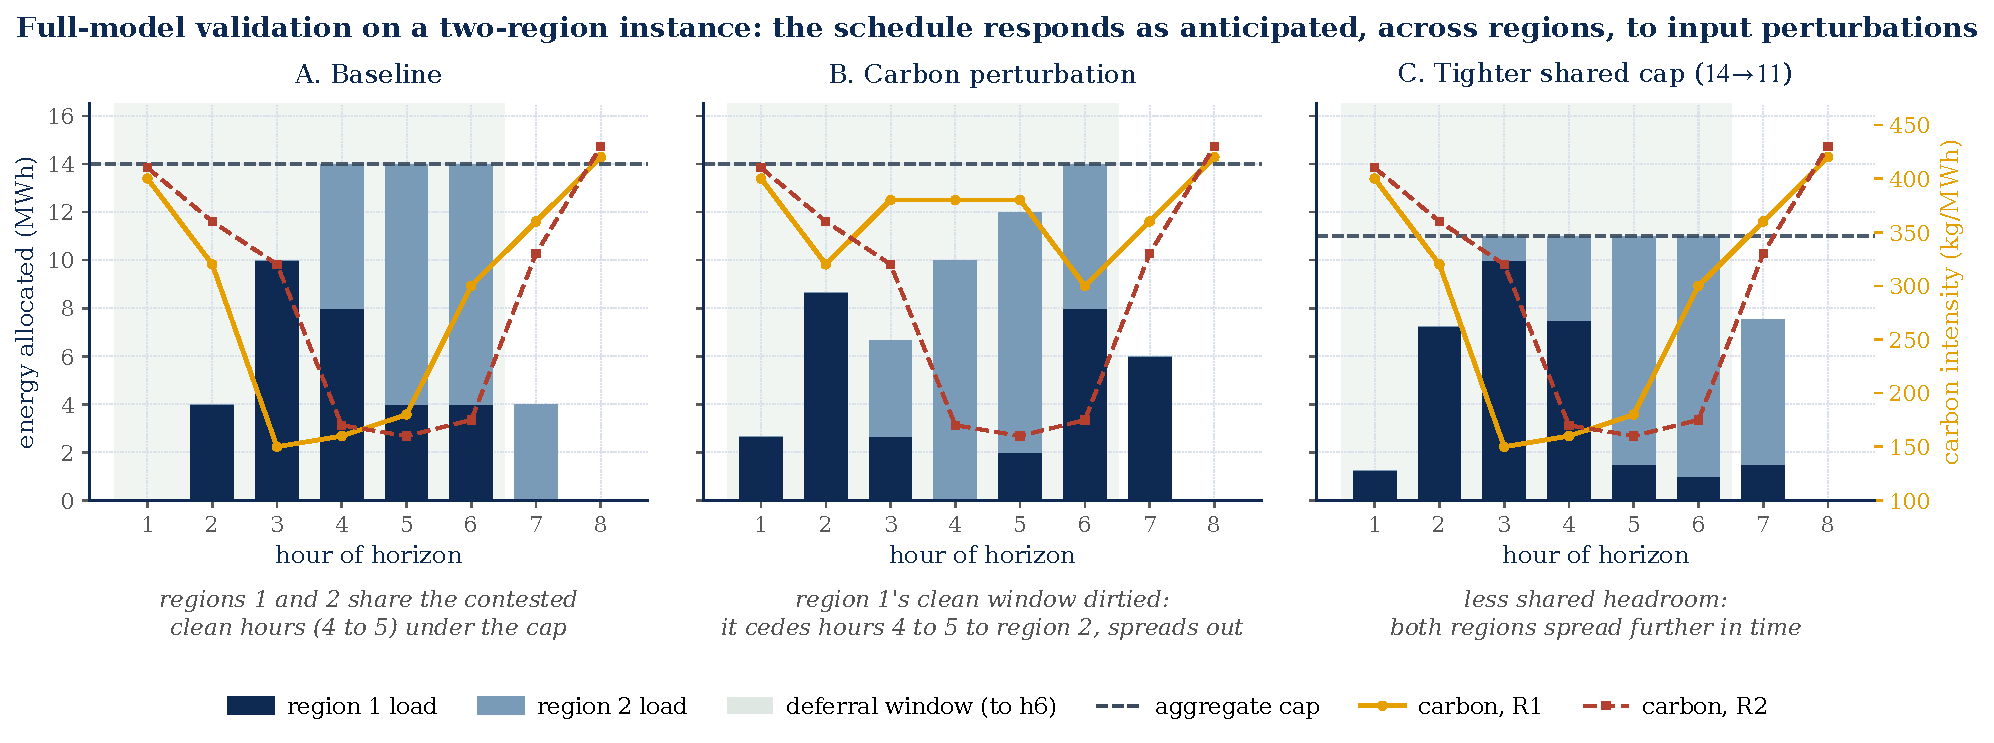
\includegraphics[width=\textwidth]{../figures/model_validation.pdf}
\caption{Full-model validation on a two-region instance. The complete feasible set
(capacity, work conservation, ramp, deferral deadline) plus a shared aggregate
hourly cap is solved jointly; stacked bars show how the two regions share each hour,
the dashed line is the aggregate cap, the curves are each region's carbon field, the
green band the deadline window. \textbf{A:} baseline, the regions split the contested
clean hours (4--5) under the cap. \textbf{B:} after dirtying region~1's clean window,
it cedes those hours to region~2 and spreads out. \textbf{C:} after tightening the
shared cap, both regions spread further in time. Each response is the one an analyst
anticipates, confirming the model encodes the intended cross-region behaviour.}
\label{fig:modelval}
\end{figure}

\subsection{The falsification test: shuffled marginals}\label{sec:test}
The scheduler is fitted twice, with covariances differing in exactly one respect:
\begin{equation}
\big(\hat\Sigma^{\mathrm{shuf}}\big)_{rs}=
\begin{cases}
\Sigma_{rr}, & r=s,\\
\mathbf{0}, & r\neq s,
\end{cases}
\label{eq:shuf}
\end{equation}
preserving every region's marginal distribution and within-region autocorrelation
while destroying only cross-region dependence. Each fitted schedule $x$ is evaluated
by the out-of-sample conditional value-at-risk of daily emissions
$e_i=\langle\rho_i,x\rangle$ realized on test day $i$; CVaR is a coherent risk
measure \citep{artzner1999} standard in stochastic programming
\citep{shapiro2009}. We use the Rockafellar--Uryasev form \citep{rockafellar2000}
\begin{equation}
\CVaR_{\beta}(e)=\min_{\tau\in\R}\;\Big\{\tau+\tfrac{1}{1-\beta}\,
\E\big[(e-\tau)_+\big]\Big\},
\qquad\beta=0.95,
\label{eq:cvar}
\end{equation}
estimated as the empirical mean of the worst $5\%$ of test days. The \emph{spatial
gap} is the difference between the two arms,
\begin{equation}
\mathrm{gap}=\CVaR_{0.95}\big(e^{\mathrm{shuf}}\big)-
\CVaR_{0.95}\big(e^{\mathrm{joint}}\big),
\label{eq:gap}
\end{equation}
positive when the joint covariance helps. The test is a falsification: it is
built to detect a spatial benefit if one exists, so a null is informative.
Figure~\ref{fig:pipeline} sketches the pipeline and Algorithm~\ref{alg:protocol}
gives the full protocol.

\begin{figure}[t]
\centering
\footnotesize
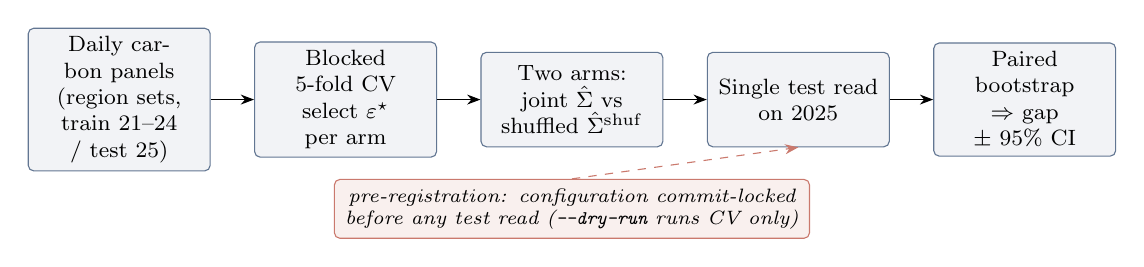
\begin{tikzpicture}[
  node distance=3.2mm and 5.5mm,
  box/.style={draw=navy!70, fill=navy!6, rounded corners=2pt, align=center,
              inner sep=3pt, text width=21mm, minimum height=12mm, font=\footnotesize},
  >=Stealth]
\definecolor{navy}{HTML}{1F3B63}
\node[box] (data) {Daily carbon panels\\(region sets,\\train 21--24 / test 25)};
\node[box, right=of data] (cv) {Blocked 5-fold CV\\select $\varepsilon^\star$\\per arm};
\node[box, right=of cv] (fit) {Two arms:\\joint $\hat\Sigma$ vs\\shuffled $\hat\Sigma^{\mathrm{shuf}}$};
\node[box, right=of fit] (test) {Single test read\\on 2025};
\node[box, right=of test] (boot) {Paired bootstrap\\$\Rightarrow$ gap\\$\pm$ 95\% CI};
\draw[->] (data)--(cv); \draw[->] (cv)--(fit); \draw[->] (fit)--(test);
\draw[->] (test)--(boot);
\node[draw=rust!70, fill=rust!8, rounded corners=2pt, below=4mm of fit,
      text width=58mm, align=center, font=\scriptsize\itshape] (lock)
      {pre-registration: configuration commit-locked before any test read
       ($\texttt{--dry-run}$ runs CV only)};
\draw[->, rust!70, dashed] (lock.north) -- (test.south);
\end{tikzpicture}
\caption{The pre-registered falsification pipeline. Cross-validation and schedule
fitting touch only the training years; the 2025 test set is read once, after the
configuration is commit-locked, and the spatial gap is read off a paired
day-bootstrap.}
\label{fig:pipeline}
\end{figure}

\begin{algorithm}[t]
\caption{Shuffled-marginals experiment (one region set)}
\label{alg:protocol}
\begin{algorithmic}[1]
\State \textbf{Input:} daily panels $\rho_{1:N}$ (train 2021--2024, test 2025);
regimes $\{$R3, R1, R2$\}$; $\alpha$-levels $\{0.30,0.50,0.75\}$; grid
$\mathcal{E}=\{0,0.1,1,10,100,1000\}$
\For{each regime, each $\alpha$, each arm $\Sigma\in\{\text{joint},
\text{shuf}\}$}
  \For{each $\varepsilon\in\mathcal{E}$}  \Comment{blocked 5-fold time-series CV}
    \For{each contiguous fold $k$}
      \State fit $\bar\rho,L$ on training folds; solve SOCP \eqref{eq:obj};
      record validation $\CVaR_{0.95}$
    \EndFor
  \EndFor
  \State $\varepsilon^\star\gets\arg\min_\varepsilon$ mean validation CVaR
  \Comment{per arm, independently}
  \State refit on full training set at $\varepsilon^\star$; evaluate
  \emph{once} on 2025 \Comment{single test read}
\EndFor
\State paired bootstrap (1000 resamples, fixed seed) on test days
$\Rightarrow$ 95\% CI for the gap \eqref{eq:gap}
\State \textbf{Pre-registration:} configuration commit-locked before any test
read; \texttt{--dry-run} gate runs CV only
\end{algorithmic}
\end{algorithm}

\subsection{Data}\label{sec:data}
Carbon intensity is hourly lifecycle intensity from Electricity Maps (academic
licence), 2021--2025, $43{,}824$ hourly observations per zone; panels are built on a
common local clock per region set, trained on 2021--2024 and tested once on 2025.
Three primary US/Canada region sets span the dependence spectrum:
\textbf{(1)}~the \emph{US West}, California, Nevada and Phoenix (CISO, BANC,
LDWP, NEVP, AZPS); \textbf{(2)}~an \emph{Ontario--Eastern belt} (CA-ON, NYISO,
MISO, PJM); and \textbf{(3)}~an \emph{engineered heterogeneous portfolio} (CISO
(solar), ERCOT (wind), BPAT (hydro)) deliberately chosen so clean periods do
\emph{not} align: the adversarial best case for diversification. Two earlier panels
corroborate: an \emph{Iberia--France} European set (ES, PT, FR), where residual
correlation collapses to the diurnal cycle, and the California/Nevada subset of the
US West before Phoenix was added at the supervisor's request. Temperature for
constraint 3b is hourly ERA5 2\,m air temperature (Open-Meteo), one load-weighted
point per zone. The licensed raw data is never committed; derived summary tables
are archived in the repository for traceability.

\subsection{Validation and mechanism diagnostics}\label{sec:diagnostics}
\paragraph{Correlation validation (RQ1).} Raw Pearson correlation conflates
co-movement with a shared diurnal cycle. We therefore report correlations of
\emph{residuals} after removing each zone's hour-of-day mean (local clock), with
overlay plots of standardized intensity for summer and winter weeks.

\paragraph{Robustness battery.} Every experiment is re-run with (i) Ledoit--Wolf
shrinkage covariance \citep{ledoit2004}; (ii) covariance estimated from seasonal
(monthly-mean) residuals; (iii) covariance from AR(1) residuals. A pre-registered
agreement rule counts a spatial effect only if positive and sign-stable across
both residual estimators. Bootstrap $p$-values across all cells receive
Benjamini--Hochberg correction at $q=0.05$ \citep{benjamini1995}; a walk-forward
refit (train 2021--2023, test 2024) checks temporal stability; a log-denser
$\varepsilon$ grid checks grid sensitivity.

\paragraph{Mean-ablation (RQ3, causal).} To test whether the mean field masks the
covariance, the mean used for \emph{scheduling} is transformed while evaluation
stays on real emissions: \textsc{level} equalizes regional time-averages (keeping
hour-of-day shape); \textsc{flat} sets a constant mean, making the mean term
constant under fixed demand, a covariance-only world in which any joint-vs-shuf
difference is attributable purely to the spatial blocks.

\paragraph{Tail dependence (RQ3, structural).} For each region pair we estimate
the upper and lower tail-dependence coefficients
$\chiU(q)=\Pr(U>q,V>q)/(1-q)$ and $\chiL(p)=\Pr(U<p,V<p)/p$ on rank
pseudo-observations of residual intensity, comparing $\chiU$ at $q=0.95$ with the
Gaussian-copula value at the matched correlation. Since the Gaussian copula, the dependence family a covariance ball can represent, is asymptotically
tail-independent \citep{embrechts2002}, a positive empirical excess would be
exploitable tail structure invisible to the DRO; and since elliptical copulas force
$\chiL=\chiU$, radial asymmetry diagnoses non-elliptical dependence.

\subsection{Phase 2: copula dependence models and a mean-dominance
bound}\label{sec:method-copula}
The covariance test answers whether \emph{elliptical} dependence helps. Because the
tail diagnostic flags \emph{non-elliptical} structure ($\chiL>\chiU$), a covariance
ball cannot by construction represent it, so a natural objection to the Phase 1
null is ``you used the wrong dependence object.'' Phase 2 forecloses that objection
by replacing the covariance ball with copula models that \emph{can} represent the
structure, and re-running the same falsification.

\paragraph{Copula-coupled resampling.} We generalize the shuffled-marginals test
from second moments to the full copula while preserving every region's empirical
marginal. Each region $r$ keeps its pool of whole daily profiles
$\{\rho^d_r\in\R^T\}$; a scenario is generated by drawing a copula sample
$u\in[0,1]^R$ and, for each region, selecting the training day whose daily-mean
intensity has rank $u_r$ (low rank $=$ clean day), then taking that day's full
profile. The copula thus governs \emph{only} the cross-region coupling, exactly as
the shuffled covariance did. Three nested fitted models span the dependence
hierarchy (a fourth, the comonotone upper bound, is added in
Section~\ref{sec:res-copula} as the ceiling):
\textbf{(i)}~the \emph{independence} copula (regions decoupled, the Phase 1
shuffled arm); \textbf{(ii)}~the \emph{Gaussian} copula at the empirical
rank-correlation (elliptical, what the covariance ball can see); and
\textbf{(iii)}~an exchangeable \emph{Clayton} copula, with lower-tail dependence
$\lambda_L=2^{-1/\theta}$ and zero upper-tail dependence \citep{joe2014}, fitted by
matching mean pairwise Kendall's $\tau$ ($\theta=2\tau/(1-\tau)$), the object
built for the $\chiL>\chiU$ finding. Clayton is sampled by Marshall--Olkin frailty;
no parametric marginal model is introduced. The exchangeable Clayton imposes a
single $\theta$ and so cannot reproduce the \emph{pair-level} heterogeneity of the
tail diagnostic (Table~\ref{tab:tails}); a regular-vine copula with edge-specific
families would. We do not fit one, for a principled reason: the comonotone arm
below realizes the supremum over \emph{all} copulas, vines included, so it
upper-bounds whatever any heterogeneous-dependence model could achieve. If the
maximal-coupling arm recovers no material value, no vine can.

\paragraph{Copula CVaR scheduler.} For each model we draw $S=1000$ scenarios
$\{\rho^s\}$ and solve the sample-average CVaR program in Rockafellar--Uryasev form
\citep{rockafellar2000},
\begin{equation}
\min_{x\in\mathcal X,\,\tau,\,z\ge0}\ \tau+\frac{1}{(1-\beta)S}\sum_{s=1}^S z_s
\quad\text{s.t.}\quad z_s\ge\langle\rho^s,x\rangle-\tau,
\label{eq:saacvar}
\end{equation}
over the \emph{same} feasible set $\mathcal X$ \eqref{eq:feasible} and regimes as
Phase 1, so the only thing that varies across arms is the dependence model. Each
schedule is evaluated once on the 2025 panel by out-of-sample $\CVaR_{0.95}$;
the reported copula gaps are $\CVaR(\text{indep})-\CVaR(\text{Gaussian})$,
$\CVaR(\text{indep})-\CVaR(\text{Clayton})$, and the asymmetry increment
$\CVaR(\text{Gaussian})-\CVaR(\text{Clayton})$, each with a paired day-bootstrap CI.
Algorithm~\ref{alg:copula} summarizes the procedure.

\begin{algorithm}[t]
\caption{Copula-scenario CVaR scheduling (one region set)}
\label{alg:copula}
\begin{algorithmic}[1]
\State \textbf{Input:} daily panels $\rho_{1:N}$ (train 2021--2024, test 2025);
dependence models $\{$independence, Gaussian, Clayton, comonotone$\}$; regimes;
$\alpha$-levels; scenarios $S=1000$, fixed seed
\For{each dependence model $C$}
  \State fit $C$ on training daily summaries (rank pseudo-observations); for Clayton,
  $\theta=2\tau/(1-\tau)$ from mean Kendall $\tau$
  \For{each regime, each $\alpha$}
    \State draw $S$ copula samples $u^s\in[0,1]^R$ \Comment{indep./Gaussian/Clayton
    frailty/comonotone}
    \State map each region's $u^s_r$ to the training day of that daily-summary rank;
    take its full profile $\Rightarrow$ scenario $\rho^s\in\R^{R\times T}$
    \Statex \hspace{1.1em}\Comment{copula-coupled resampling: marginals exact,
    only cross-region coupling changes}
    \State solve the CVaR-SAA program \eqref{eq:saacvar} over $\mathcal X$
    $\Rightarrow$ schedule $x$
    \State evaluate \emph{once} on 2025 $\Rightarrow$ out-of-sample $\CVaR_{0.95}$
  \EndFor
\EndFor
\State copula gaps vs.\ independence $+$ paired day-bootstrap CIs; comonotone
realizes $\sup_C$, the ceiling $\Lambda$
\end{algorithmic}
\end{algorithm}

\paragraph{Why the dependence model is second-order.} Two facts make the
dependence model second-order to the mean field. The first is a decomposition: by
the translation invariance of CVaR, writing the carbon field as mean plus zero-mean
residual $\rho=\bar\rho+\xi$ and noting $\langle\bar\rho,x\rangle$ is deterministic,
\begin{equation}
\CVaR_\beta\!\big(\langle\rho,x\rangle\big)=
\underbrace{\langle\bar\rho,x\rangle}_{\text{dependence-independent}}+\;
\CVaR_\beta\!\big(\langle\xi,x\rangle\big),
\label{eq:meandom}
\end{equation}
so for a \emph{fixed} schedule the dependence model moves only the residual term.
The second is an a-priori bound on how far it can move the \emph{optimal} value.

\begin{proposition}[Spatial gap control, SOCP]\label{prop:meandom}
Let $\mathrm{OPT}(\Sigma)$ be the optimal value of the SOCP \eqref{eq:socp} for a
covariance $\Sigma$, and let $\Sigma^{\mathrm{shuf}}$ be its block-diagonal
(cross-region-zeroed) counterpart with $\Sigma^{\mathrm{off}}=\Sigma-
\Sigma^{\mathrm{shuf}}$. Then the spatial gap obeys
\begin{equation}
\big|\mathrm{OPT}(\Sigma)-\mathrm{OPT}(\Sigma^{\mathrm{shuf}})\big|\ \le\
\varepsilon\,\Big(\max_{x\in\mathcal X}\lVert x\rVert_2\Big)\,
\big\lVert\Sigma^{\mathrm{off}}\big\rVert_2^{1/2},
\label{eq:propbound}
\end{equation}
which vanishes as $\varepsilon\to0$ (no robustification) or
$\Sigma^{\mathrm{off}}\to0$ (no cross-region structure).
\end{proposition}

\begin{proof}
The two programs share the feasible set $\mathcal X$ and differ only in the conic
penalty. For fixed $x$, using $|\sqrt a-\sqrt b|\le\sqrt{|a-b|}$ and the Rayleigh
bound $|x^\top\Sigma^{\mathrm{off}}x|\le\lVert\Sigma^{\mathrm{off}}\rVert_2\lVert
x\rVert_2^2$,
\[
\big|\varepsilon\sqrt{x^\top\Sigma x}-\varepsilon\sqrt{x^\top\Sigma^{\mathrm{shuf}}x}\big|
\le\varepsilon\sqrt{|x^\top\Sigma^{\mathrm{off}}x|}
\le\varepsilon\lVert x\rVert_2\lVert\Sigma^{\mathrm{off}}\rVert_2^{1/2}.
\]
Since the infimum is $1$-Lipschitz in the sup-norm of the objective, two objectives
that differ pointwise by at most $\delta$ over a common feasible set have optimal
values differing by at most $\delta$. The feasible set $\mathcal X$ is a bounded
polytope (the capacity bounds C0), hence compact, so $\max_{x\in\mathcal X}\lVert
x\rVert_2$ is attained; taking that maximum gives \eqref{eq:propbound}.
\end{proof}

\noindent The bound is a conservative \emph{certificate}, not a tight prediction.
Evaluated on each grid's training covariance (with $\varepsilon^\star=1$, the
a-priori feasible bound $\max_{x}\lVert x\rVert_2=\bar x\sqrt{R\,T\,u}$ where $\bar
x$ is the per-cell cap and $u$ the utilization, and $\lVert\Sigma^{\mathrm{off}}
\rVert_2$ the spectral norm of the destroyed cross-region blocks), its right-hand
side is $7.4\%$ (Eastern US--Canada), $9.6\%$ (Diversified) and $12.7\%$ (Western
US) of $\CVaR_{0.95}$; the realized gaps (Table~\ref{tab:gaps}) never exceed
$0.23\%$, two orders of magnitude smaller. The theorem therefore caps the spatial
gap at the few-percent scale \emph{before any experiment is run}, and the
experiments then pin it far below that cap. What the bound buys is not tightness but
structure: the spatial gap is governed by $\varepsilon$ and the cross-region block
norm, and is forced to zero in the no-robustification and no-cross-structure limits.
Most of the remaining slack lives in the feasible-diameter factor $\max_x\lVert
x\rVert_2$, an a-priori worst case; substituting the realized optimal $\lVert
x^\star\rVert_2$ would tighten the certificate considerably, at the cost of making it
post-hoc rather than a-priori. We keep the a-priori form deliberately, since its
purpose is to bound the gap \emph{before} the experiment, not to predict it. The
\emph{tight} ceiling is measured, not bounded: the comonotone arm of
Section~\ref{sec:res-copula} realizes the supremum over copulas, and across scenario
seeds its gain is centred on zero with $|\Lambda|\lesssim0.1\%$ of $\CVaR_{0.95}$, at
the sampling-noise floor. The mean-ablation of Section~\ref{sec:res-ablation}
bounds the same quantity from a second, independent angle. Both put $\Lambda$ an
order of magnitude below the schedule's mean-driven value; hence the mean field pins
the schedule and the dependence model, elliptical or not, is immaterial. The prediction that even Clayton cannot recover material
value is confirmed in Section~\ref{sec:res-copula}.

\paragraph{Computational considerations.} Each instance is small: the decision
vector has $RT\le 5\times24=120$ entries and the feasible set adds $O(RT)$ linear
constraints, so the SOCP \eqref{eq:socp} solves in $0.19$--$0.26$\,s and the
CVaR-SAA LP \eqref{eq:saacvar}, which appends $S=1000$ epigraph variables and
constraints, in $0.9$--$1.3$\,s (median over five repetitions, CLARABEL/HiGHS,
commodity laptop). The cost is in the \emph{number} of instances, not their size:
one region-set experiment solves $3\text{ regimes}\times3\,\alpha\times2\text{
arms}\times(6\,\varepsilon\times5\text{ folds}+1\text{ test read})=558$ SOCPs, and
the full Phase 1 battery (region sets $\times$ \{sample, Ledoit--Wolf, seasonal,
AR(1), two ablations, walk-forward, fine grid\}) is on the order of $10^4$ SOCP
solves; Phase 2 adds $3\times3\times3\times4=108$ CVaR-SAA LPs. Total wall-clock for
the entire study is under two hours on one core, so reproduction is cheap.

\subsection{Reproducibility}\label{sec:repro}
All code is version-controlled (private repository, continuous-integration test
suite, $184$ unit tests, including a feasible-set equivalence test pinning the
Phase 2 CVaR scheduler to the Phase 1 constraint set); experiment configurations
are commit-locked before test-set evaluation; bootstrap and scenario seeds are
fixed; and every number reported in
Sections~\ref{sec:results}--\ref{sec:discussion} traces to an archived summary
table. Solvers: CLARABEL/ECOS for the SOCP; HiGHS for the CVaR-SAA linear programs
and deterministic LP baselines.

% ===================== 4. RESULTS (RUN 2) =====================
\section{Results}\label{sec:results}

\subsection{The spatial assumption is valid (RQ1)}\label{sec:res-corr}
The premise holds. After removing each zone's hour-of-day mean,
cross-region correlations of carbon intensity in the two electrically coupled
US/Canada cases are strong and survive de-seasonalization: in the US West,
CISO--NEVP $0.78$ and CISO--LDWP $0.72$ (shared solar resource and weather across
WECC); in the Ontario--Eastern belt, CA-ON--NYISO $0.73$ and MISO--PJM $0.70$
(weather fronts traversing the Eastern Interconnection). The engineered
heterogeneous portfolio behaves as designed: ERCOT--BPAT residual correlation is
$0.00$, with CISO--BPAT at $0.33$. Figure~\ref{fig:heatmaps} shows the residual
correlation matrices; overlay plots of standardized intensity (archived with the
code) confirm visible co-movement in summer and winter weeks for the coupled
cases. Together with the corroborating panels, the California/Nevada subset
($0.65$--$0.78$ within-state) and Iberia--France, the cases span the dependence
spectrum from $\approx 0$ to $\approx 0.8$, so whatever the scheduling result, it
cannot be attributed to an absence of correlation in the data.

\begin{figure}[t]
\centering
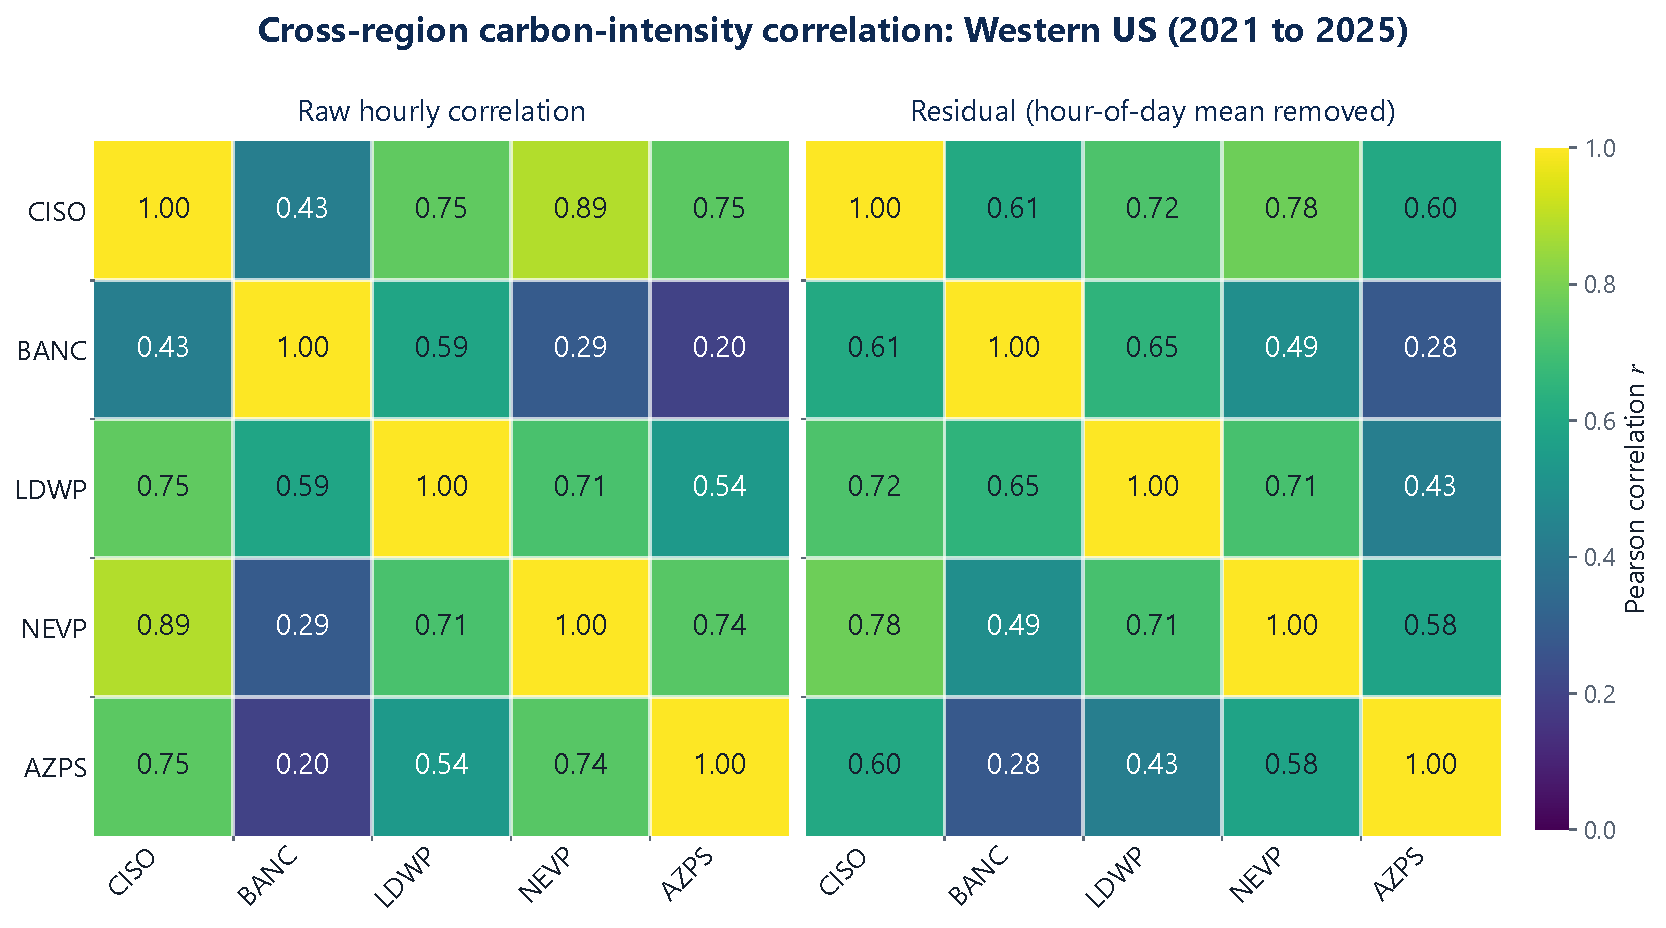
\includegraphics[width=0.48\textwidth]{../figures/ci_corr_heatmap_us_west.pdf}\hfill
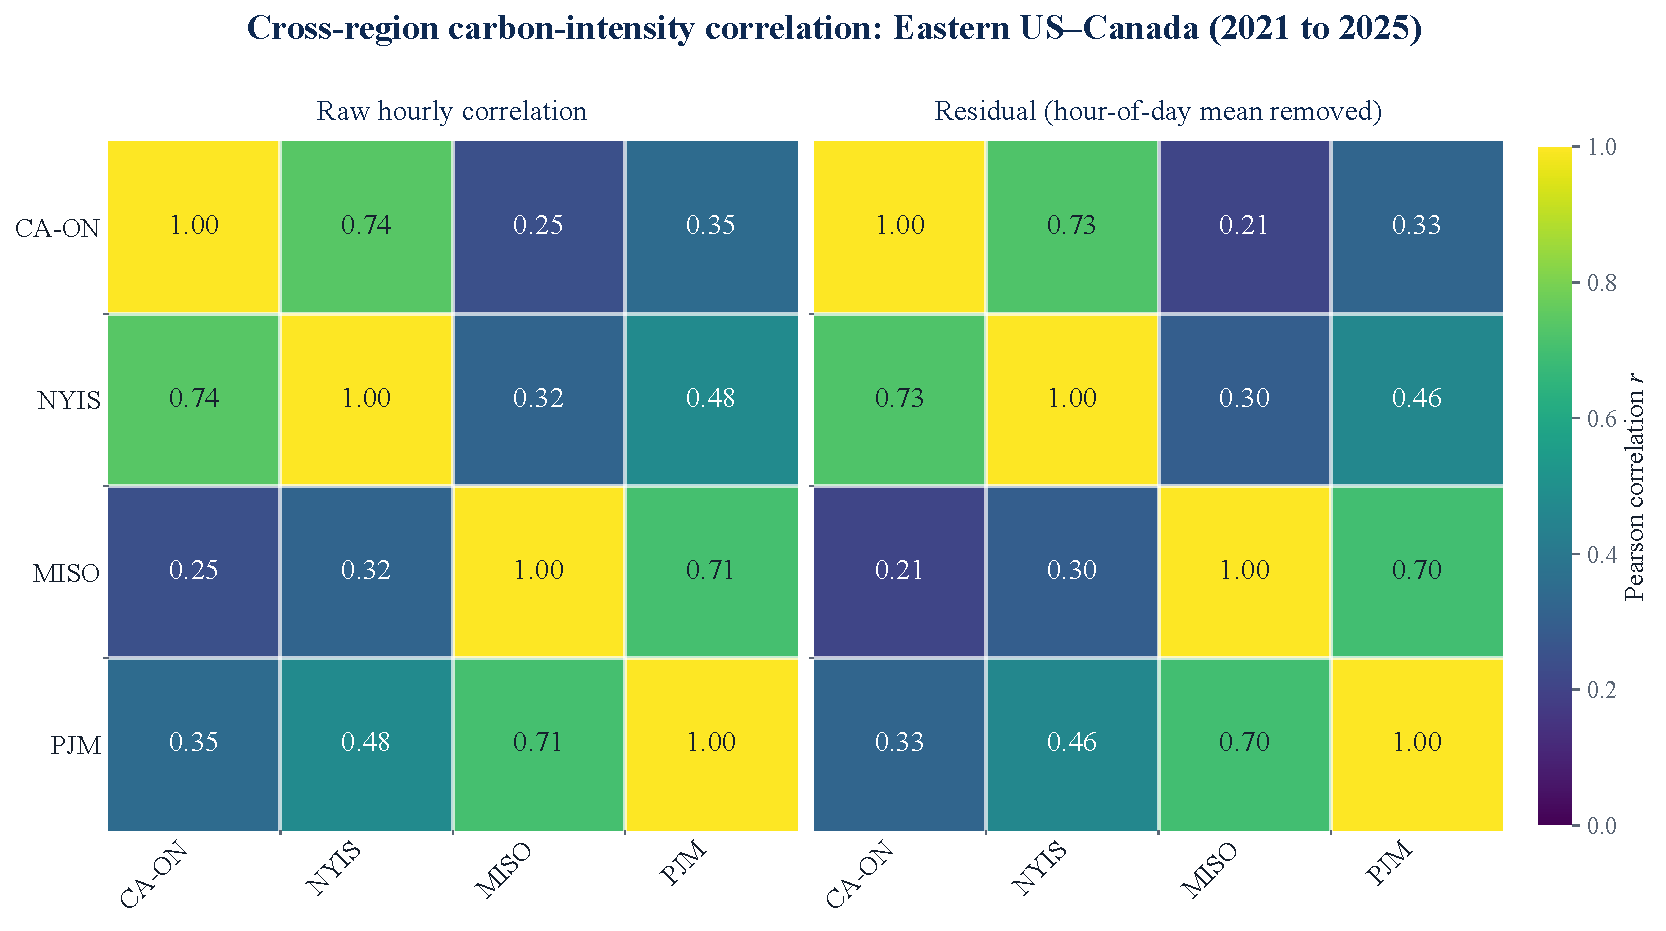
\includegraphics[width=0.48\textwidth]{../figures/ci_corr_heatmap_taskc.pdf}
\caption{Residual (hour-of-day-removed) cross-region correlation of hourly carbon
intensity, 2021--2025. Left: US West (CISO, BANC, LDWP, NEVP, AZPS). Right:
Ontario--Eastern belt (CA-ON, NYISO, MISO, PJM). Spatial correlation is strong and
genuine in both, the assumption motivating spatial DRO is empirically valid.}
\label{fig:heatmaps}
\end{figure}

Figure~\ref{fig:map} places the three grids geographically and draws each
within-grid residual correlation as a weighted edge. The picture matches the
physics: the US West forms one tightly-coupled WECC cluster, the Ontario--Eastern
belt another along the Eastern Interconnection, while the engineered portfolio
spans the continent with thin (near-zero) edges by construction.

\begin{figure}[t]
\centering
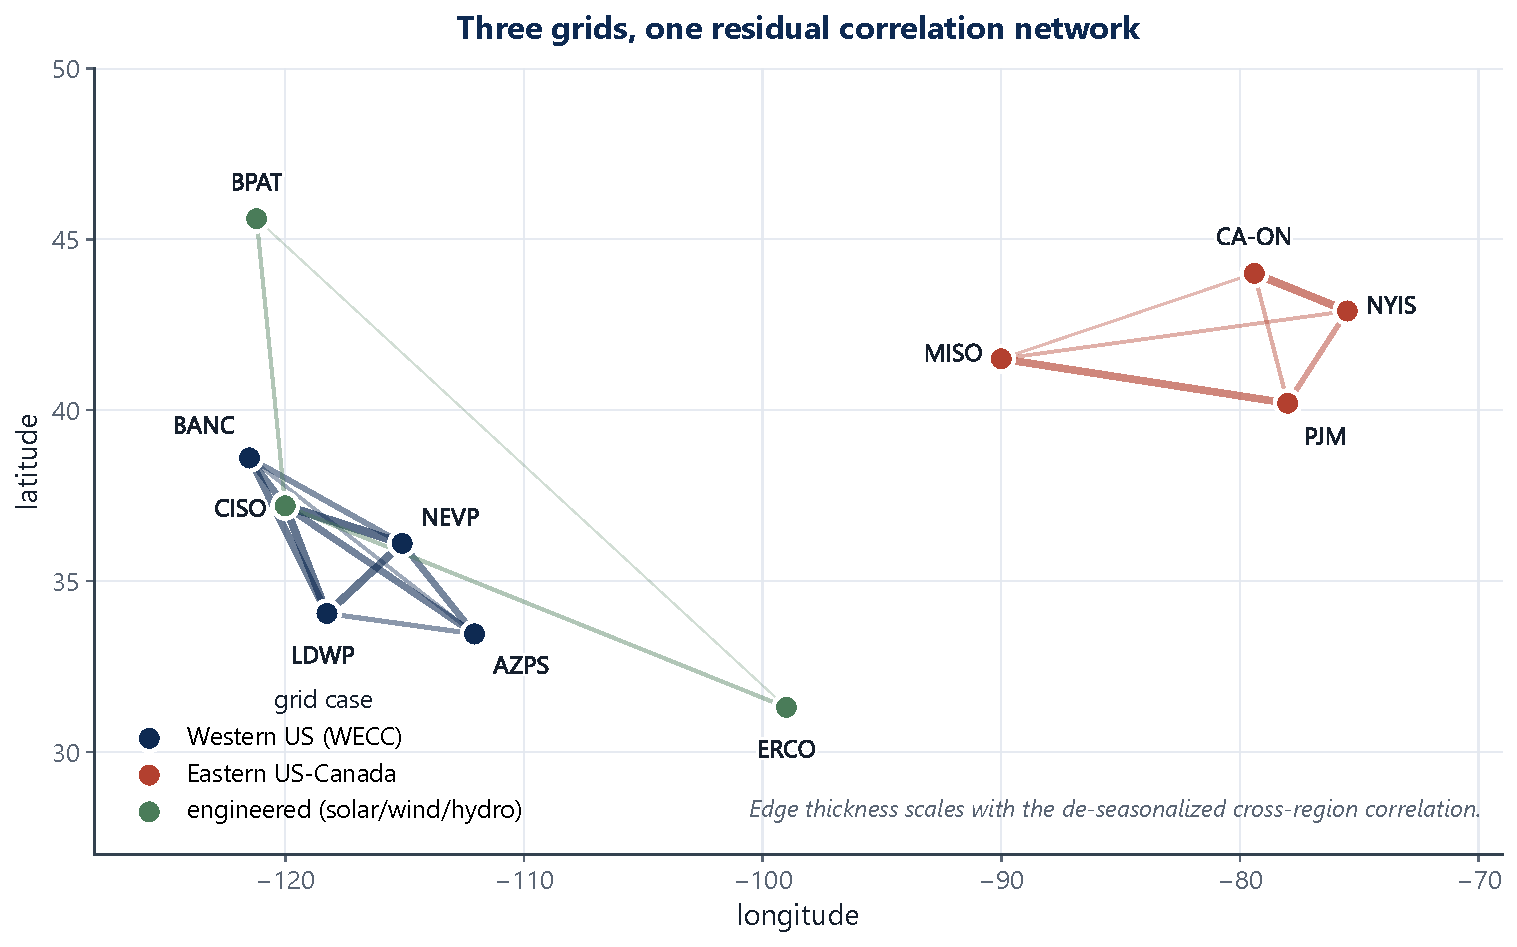
\includegraphics[width=0.92\textwidth]{../figures/correlation_map.pdf}
\caption{The three grids and their residual correlation network. Nodes are
Electricity Maps zones at their geographic centroids; edge weight is the
de-seasonalized cross-region correlation. Tight clusters (US West, Ontario--Eastern
belt) contrast with the deliberately diversified engineered portfolio.}
\label{fig:map}
\end{figure}

\subsection{The spatial gap is null across the spectrum (RQ2)}\label{sec:res-gap}
Table~\ref{tab:gaps} reports the spatial gap \eqref{eq:gap} for the three
pre-registered US/Canada cases: nine cells each (three constraint regimes $\times$
three $\alpha$-levels), CV-selected $\varepsilon^\star$, single test read on 2025.
The gap never exceeds a few tenths of one percent of test
$\CVaR_{0.95}$ in either direction. Where the bootstrap calls a cell
``detectable'' the effect is genuine but economically negligible (on the order
of a few hundred $\gco$ out of a $\CVaR$ of $1.5\times10^6$) and, decisively, its
\emph{sign} flips across adjacent $\alpha$-levels within the same regime. A
consistently exploitable spatial structure would not reverse direction under a
change of the flexible-load fraction; these reversals are the signature of
optimization at the boundary of materiality, not of a usable effect. (We confirmed
the detectable cells are not numerical: re-solving with CLARABEL and SCS reproduces
the gap to four significant figures, so the sign instability is in the data, not the
solver.) The California/Nevada panel agrees (gaps in $[-0.012,+0.058]\%$, DRO active
throughout).

Crucially, this is a null of the \emph{strong} kind. In all three pre-registered
cases cross-validation \emph{chooses} a non-trivial ambiguity radius:
$\varepsilon^\star=1$ in every one of the 27 cells for Eastern US--Canada and
Diversified, and in 25 of 27 for Western US. The DRO is therefore
genuinely engaged (it is paying for robustness, not collapsing to the nominal
problem) and the two arms still coincide. A null in which CV had selected
$\varepsilon^\star=0$ would be uninformative (robustification switched off, so the
arms must match by construction); here the robustification is demonstrably on and
the spatial covariance still buys nothing. This is the first regime in the project
where the DRO is consistently active, which is precisely what makes the null
informative rather than vacuous. Figure~\ref{fig:cvcurve} shows the cross-validation
curves directly: validation $\CVaR_{0.95}$ dips to an interior minimum at a
non-trivial $\varepsilon^\star$ before rising as over-conservatism sets in, and the
joint and shuffled curves lie on top of one another.

\begin{figure}[t]
\centering
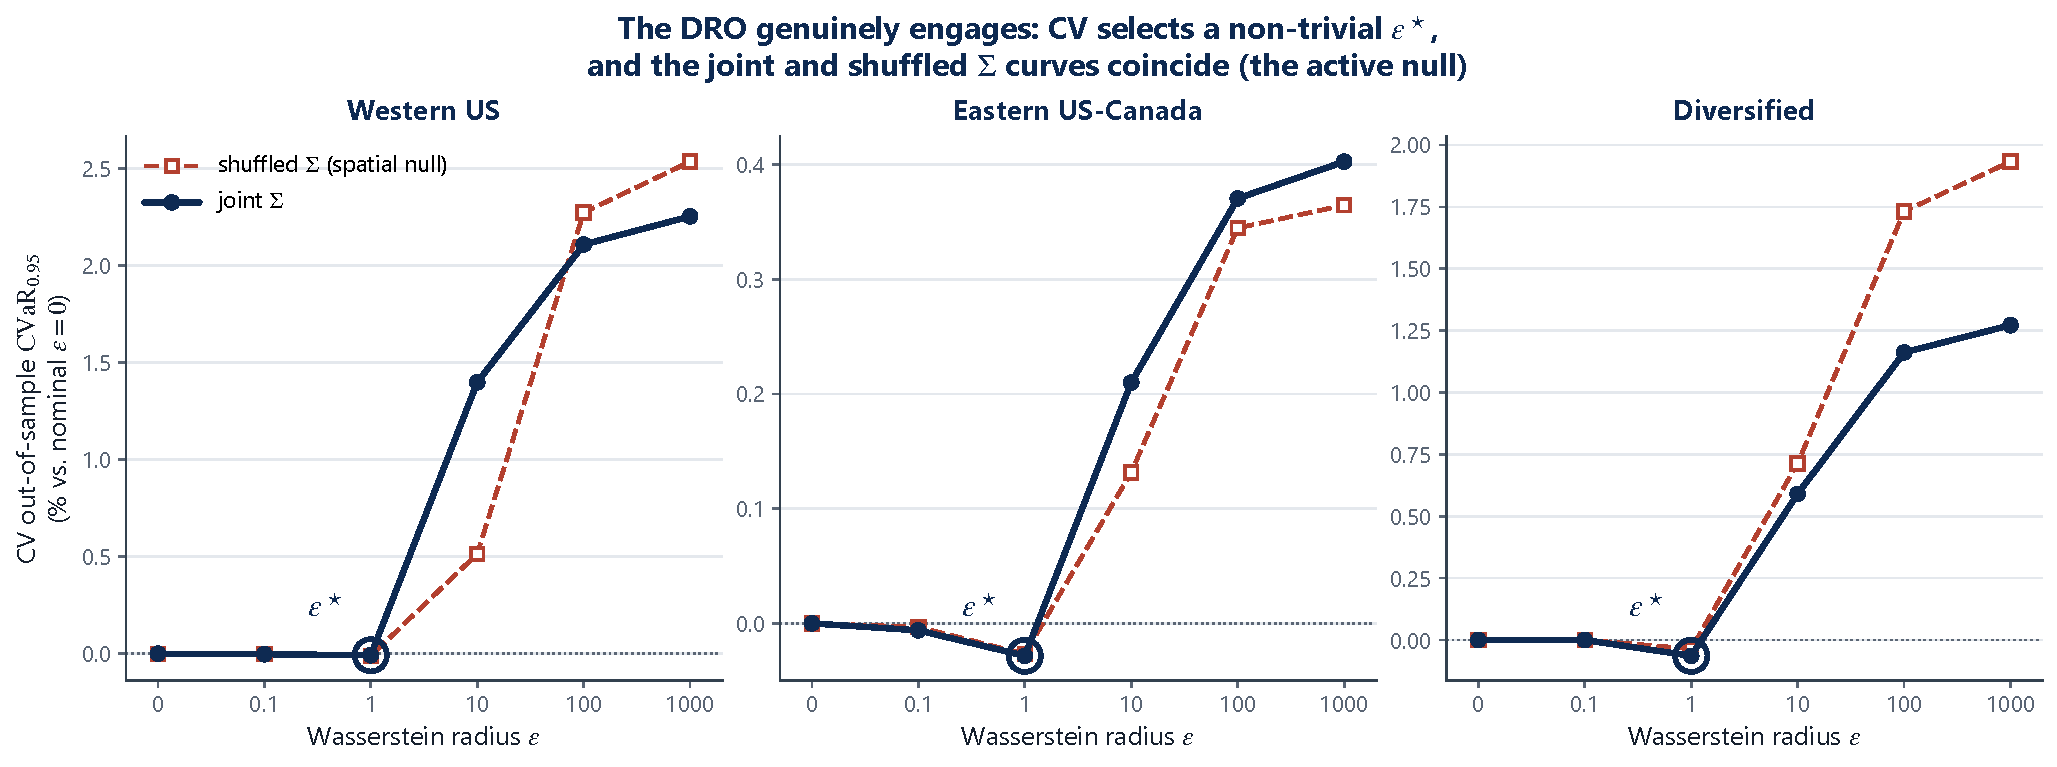
\includegraphics[width=\textwidth]{../figures/cv_curve.pdf}
\caption{The DRO genuinely engages. Blocked 5-fold cross-validation
$\CVaR_{0.95}$ (relative to the nominal $\varepsilon=0$ problem) against the
Wasserstein radius $\varepsilon$, for the joint (solid) and shuffled (dashed)
covariances. Cross-validation selects an interior $\varepsilon^\star$ (circled),
not $\varepsilon=0$, so the robustification is on; the two curves coincide, so the
spatial covariance changes nothing. Large $\varepsilon$ is over-conservative.}
\label{fig:cvcurve}
\end{figure}

The Iberia--France panel is the instructive contrast and the project's historical
starting point. There the residual correlation is near zero, and CV does not even
consistently engage the DRO: $\varepsilon^\star$ flickers between $0$, $0.1$, $1$
and $10$ across cells, collapsing to $0$ in several. This is itself consistent with
the thesis (where there is no cross-region structure, the machinery sees nothing
worth robustifying) but it makes the Iberian null the \emph{weak} kind. We
therefore retain it only as low-correlation, real-grid external validity, and rest
the central claim on the US/Canada cases where the DRO is unambiguously on. The
engineered Diversified portfolio supplies the strong zero-correlation null
($\varepsilon^\star=1$ throughout, still no value) that Iberia cannot.

\begin{table}[t]
\centering\small
\caption{Spatial gap (\% of test $\CVaR_{0.95}$; positive $=$ joint covariance
better) for the three US/Canada cases. R3 $=$ reference regime, R1 $=$ $+$deadline,
R2 $=$ $+$variable carbon-coupled capacity. ``det.''\ $=$ bootstrap 95\% CI
excludes zero.}
\label{tab:gaps}
\begin{tabular}{llrrrrrr}
\toprule
& & \multicolumn{2}{c}{Diversified ($\bar r\approx0$)} &
\multicolumn{2}{c}{Eastern US--Canada ($\bar r\approx0.5$)} &
\multicolumn{2}{c}{Western US ($\bar r\approx0.5$)}\\
\cmidrule(lr){3-4}\cmidrule(lr){5-6}\cmidrule(lr){7-8}
Regime & $\alpha$ & gap\,\% & det. & gap\,\% & det. & gap\,\% & det.\\
\midrule
R3 & 0.30 & $-0.233$ & \checkmark & $-0.022$ & \checkmark & $+0.043$ & \\
R3 & 0.50 & $-0.177$ & \checkmark & $-0.002$ &  & $+0.032$ & \\
R3 & 0.75 & $+0.001$ &  & $+0.034$ & \checkmark & $-0.005$ & \\
R1 & 0.30 & $-0.233$ & \checkmark & $-0.022$ & \checkmark & $+0.014$ & \\
R1 & 0.50 & $-0.177$ & \checkmark & $-0.002$ &  & $+0.028$ & \\
R1 & 0.75 & $+0.001$ &  & $+0.034$ & \checkmark & $+0.002$ & \\
R2 & 0.30 & $-0.211$ & \checkmark & $+0.038$ & \checkmark & $+0.008$ & \\
R2 & 0.50 & $-0.154$ & \checkmark & $+0.030$ & \checkmark & $+0.005$ & \\
R2 & 0.75 & $+0.062$ & \checkmark & $+0.009$ &  & $+0.000$ & \checkmark\\
\bottomrule
\end{tabular}
\end{table}

Three readings of Table~\ref{tab:gaps} matter. First, in the adversarial
diversification case (Diversified) the joint covariance actually
\emph{hurts} at low $\alpha$ (up to $-0.23\%$): with no true cross-structure, the
joint estimator fits noise that the block-diagonal arm is spared. Second, in the
strongly correlated belt (Eastern US--Canada) the detectable cells flip sign between
$\alpha=0.30$ and $\alpha=0.75$ within the same regime. Third, the US West (strongest correlation of all) produces no detectable cell beyond one of
magnitude $+3\times10^{-6}\%$. Figure~\ref{fig:finding}A plots all 27 cells
against each case's mean residual correlation: the cloud stays on zero across the
whole correlation range. \textbf{Validity of the spatial assumption does not imply
value from it.}

\begin{figure}[t]
\centering
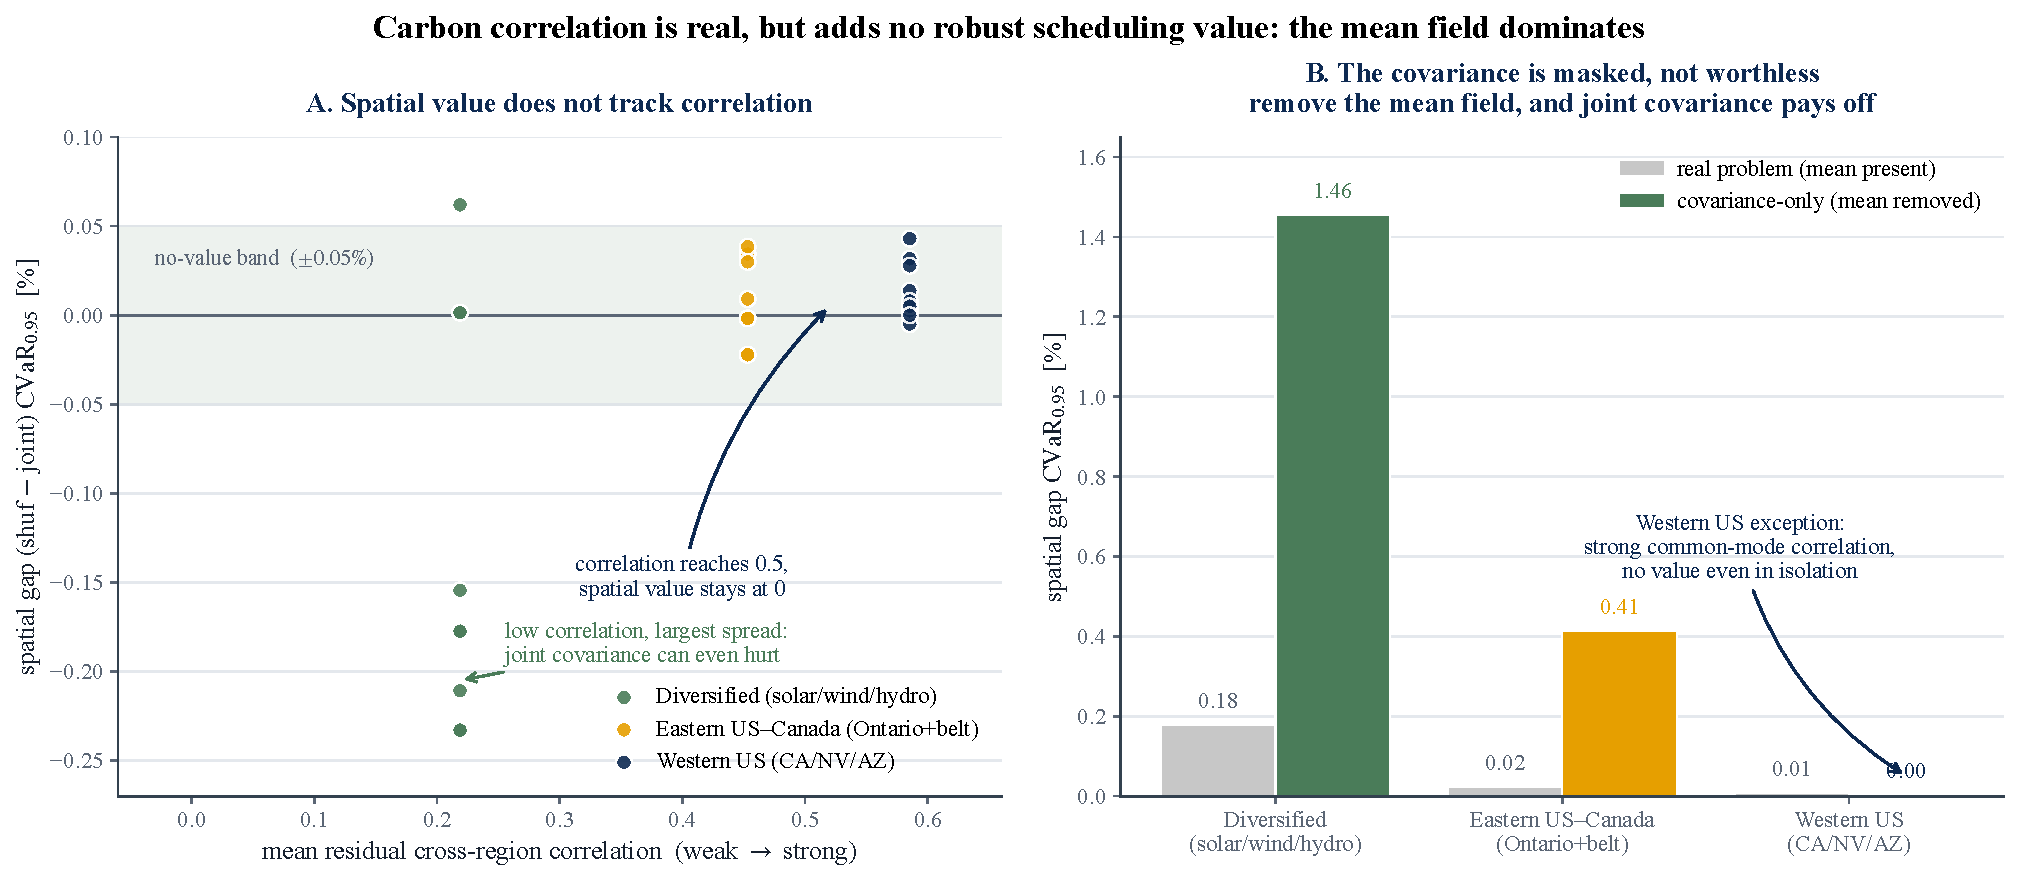
\includegraphics[width=\textwidth]{../figures/finding.pdf}
\caption{The Phase 1 finding. \textbf{A:} spatial gap vs.\ mean residual
cross-region correlation; value does not track correlation anywhere on the
spectrum. \textbf{B:} mean-ablation; in the covariance-only world (constant
scheduling mean) the joint covariance pays off by up to $+1.46\%$, proving the
spatial signal is real but \emph{masked} by the mean carbon field, not absent.}
\label{fig:finding}
\end{figure}

The null is visible in the schedules themselves. Figure~\ref{fig:schedule} overlays
the optimal load for the joint and shuffled covariances on each region's mean carbon
field: the two schedules are indistinguishable to the eye, and both place compute in
the cleaner hours subject to the deadline and ramp constraints. Destroying the
cross-region covariance changes essentially nothing about what the scheduler does.

\begin{figure}[t]
\centering
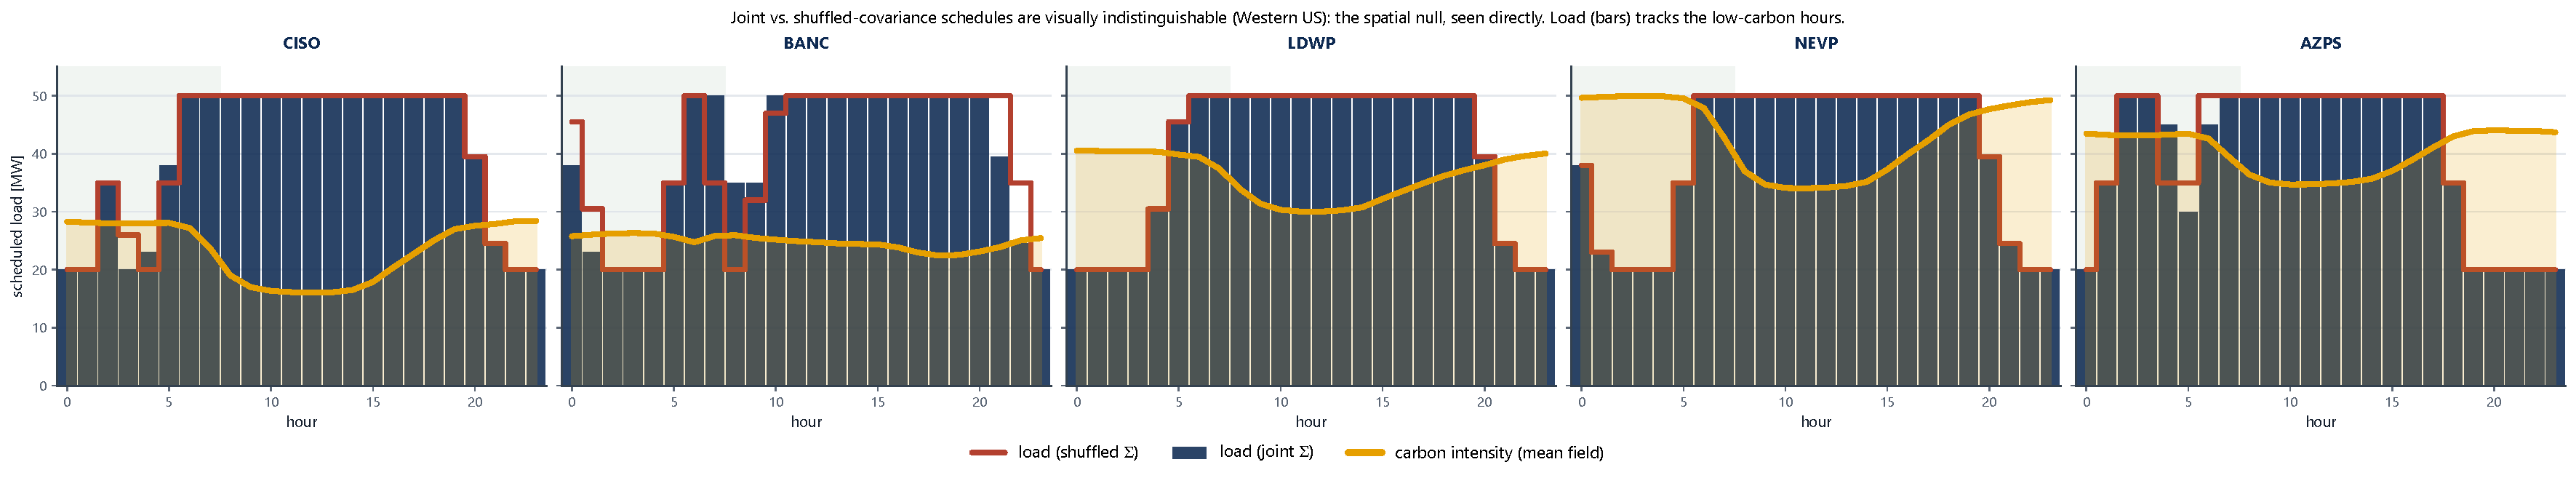
\includegraphics[width=\textwidth]{../figures/schedule_us_west.pdf}
\caption{The spatial null, seen directly (Western US, regime R3,
$\alpha=0.5$, $\varepsilon^\star=1$). Bars are the optimal load under the joint
covariance; the red step is the load under the shuffled (block-diagonal)
covariance. The two coincide. The gold curve is each region's mean carbon
intensity; the green band marks the deadline window $[0,7]$.}
\label{fig:schedule}
\end{figure}

\subsection{The null survives a pre-registered robustness battery
(RQ2)}\label{sec:res-robust}
Table~\ref{tab:robust} summarizes. Re-estimating the covariance with Ledoit--Wolf
shrinkage, seasonal residuals, or AR(1) residuals never produces a spatial effect
that passes the pre-registered agreement rule (positive and sign-stable across
both residual estimators). The largest battery value anywhere, $+0.179\%$ (AR(1),
Eastern US--Canada, $\alpha=0.30$), appears \emph{only} under AR(1) and not under the
seasonal estimator, so the rule rejects it. Benjamini--Hochberg correction at
$q=0.05$ across all 144 non-ablation cells (four grid-runs, the three primary grids
plus the locked Task~C replication, each at $3\text{ regimes}\times3\,\alpha=9$ cells
under the four covariance estimators \{sample, Ledoit--Wolf, seasonal, AR(1)\}:
$4\times9\times4=144$) leaves that same already-rejected cell as the largest
surviving positive gap; nothing material survives both filters.
A walk-forward refit (train 2021--2023, test 2024) reproduces the null out of
time: maximum absolute gap $0.036\%$ (Eastern US--Canada), $0.028\%$
(Western US), $0.217\%$ (Diversified, again negative). An
11-point log-denser $\varepsilon$ grid changes no gap at the reported precision.
Finally, a \emph{constraint-tightness} sensitivity directly probes the most
plausible route to spatial value: tripling the binding tightness of the ramp limit
($\Delta_r=5$ instead of $15$ MW/h) shrinks the feasible set so the schedule has far
less freedom to track the mean field, yet the null is unmoved, with maximum
absolute gap $0.028\%$ (Western US), $0.044\%$ (Eastern US--Canada) and $0.169\%$
(Diversified), all sign-flipping and with $\varepsilon^\star=1$ retained.
The covariance does not begin to pay even when the mean's pull is mechanically
curtailed. A complementary \emph{utilization} sweep makes the same point through the
workload: raising daily utilization from the baseline $80\%$ to $95\%$ packs the
facility near capacity and strips out almost all scheduling freedom, yet the gap
only \emph{shrinks} (maximum absolute gap $0.017\%$ for Western US, $0.048\%$ for
Eastern US--Canada, $0.071\%$ for Diversified), and at a loose $50\%$ it stays
immaterial ($\le0.25\%$); $\varepsilon^\star=1$ throughout. Across the full
$\{50,80,95\}\%$ range the null is unmoved. Figure~\ref{fig:robust} collects the
covariance-estimator and temporal battery: across all six arms and three grids,
every spatial gap sits inside the no-value band.

\paragraph{Tail level: the null holds from $\CVaR_{0.90}$ to $\CVaR_{0.99}$.}
The primary read fixes the tail at $\beta=0.95$. Because the residual co-movement
lives in the \emph{clean} tail (Section~\ref{sec:res-tails}), the natural worry is
that spatial value might surface only at a deeper risk level. Re-running the full
pipeline (cross-validated $\varepsilon$, single 2025 read) at
$\beta\in\{0.90,0.95,0.99\}$ rejects this (Table~\ref{tab:cvarsweep}). The DRO stays
engaged ($\varepsilon^\star=1$ almost everywhere) and the gap stays immaterial at
every level. Probing the deepest tail widens the magnitudes slightly but never to
materiality: the largest \emph{positive} gap anywhere is $+0.14\%$ (Western US,
$\beta=0.99$), still a third of the $0.4\%$ margin and not sign-stable, while in the
adversarial Diversified grid the joint covariance becomes \emph{more} negative at
$\beta=0.99$ ($-0.36\%$, i.e.\ it hurts), exactly as the noise-fitting account
predicts. Deepening the tail, the regime where elliptical-blind tail dependence
should matter most, does not turn the covariance on.
The $\beta=0.99$ estimates are necessarily noisier, since the tail thins to a handful
of days: the per-cell paired-bootstrap standard error rises to $0.15\%$ for Western
US (against $\le0.04\%$ at $\beta=0.90$), so that grid's largest $\beta=0.99$ point
estimate ($+0.14\%$) is itself within one standard error of zero. The apparent
widening at the deepest tail is sampling noise, not emerging spatial value. This
sweep is reported as a descriptive robustness check, \emph{outside} the
pre-registered $144$-cell FDR family of Table~\ref{tab:robust}; for completeness, no
sweep cell produces a gap that is both positive and materially large (every
detectable cell is either negative or below the $0.4\%$ margin), so none would
survive multiple-testing correction as a discovery.

\begin{table}[h]
\centering\small
\caption{Spatial gap range (min, max over the nine cells, \% of test
$\CVaR_\beta$) at three tail levels. The DRO is engaged ($\varepsilon^\star=1$
almost everywhere) throughout. No level yields a sign-stable positive gap reaching
the $0.4\%$ materiality margin.}
\label{tab:cvarsweep}
\begin{tabular}{lccc}
\toprule
Grid & $\beta=0.90$ & $\beta=0.95$ & $\beta=0.99$\\
\midrule
Western US         & $[-0.04,+0.01]$ & $[-0.01,+0.04]$ & $[\phantom{-}0.00,+0.14]$\\
Eastern US--Canada & $[-0.02,+0.04]$ & $[-0.02,+0.04]$ & $[-0.01,+0.09]$\\
Diversified        & $[-0.23,+0.08]$ & $[-0.23,+0.06]$ & $[-0.36,+0.02]$\\
\bottomrule
\end{tabular}
\end{table}

\paragraph{The null is not a conditioning artifact.} Block-diagonalizing $\Sigma$
also changes its conditioning, so one might worry the null reflects the joint arm
being harder to estimate rather than the cross-structure being valueless. The two
arms are conditioned to the same order (ridge-regularized $\kappa\approx
1.1$--$1.6\times10^5$ for the joint covariance, $0.4$--$0.8\times10^5$ for the
shuffled, the joint arm somewhat higher as expected for the richer model). The
mean-ablation of Section~\ref{sec:res-ablation} is the decisive control: it reuses
the \emph{same} joint $\Sigma$ at the \emph{same} conditioning and, removing only
the mean field, the covariance recovers up to $+1.46\%$. Estimation conditioning
therefore cannot be what suppresses the spatial value; the mean field is.

\begin{figure}[t]
\centering
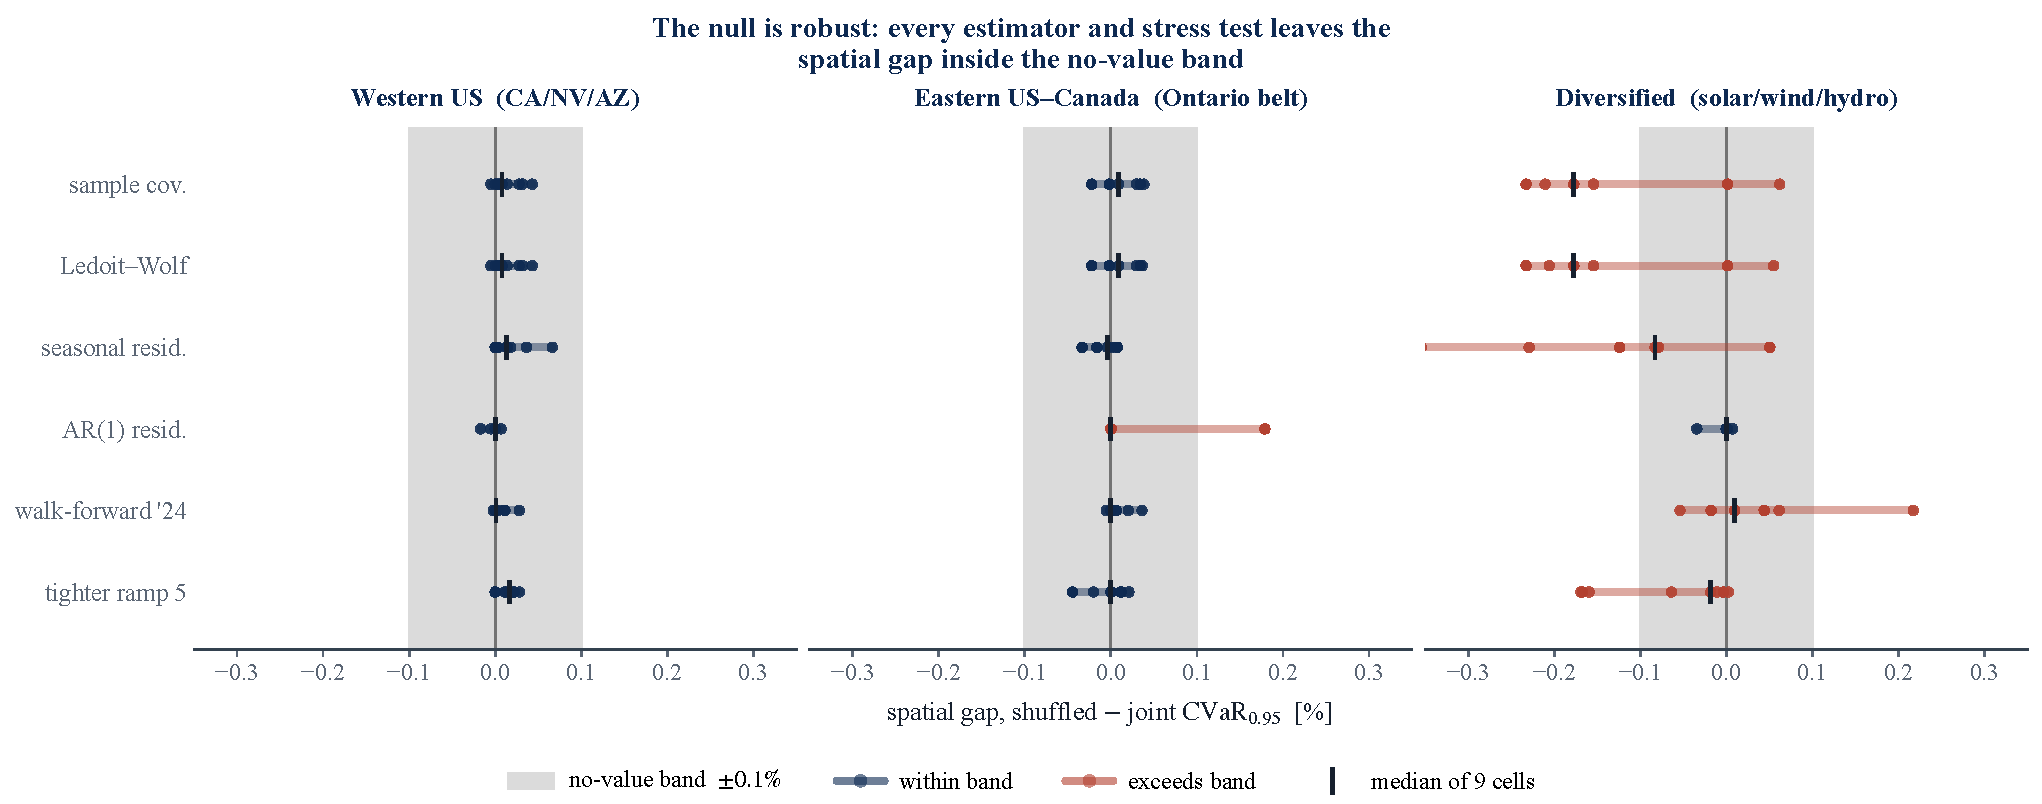
\includegraphics[width=\textwidth]{../figures/robustness.pdf}
\caption{Robustness of the null. For each grid and each robustness arm (sample
covariance, Ledoit--Wolf, seasonal and AR(1) residuals, walk-forward to 2024, and a
$3\times$ tighter ramp), dots are the spatial gap for the nine (regime,~$\alpha$)
cells and the tick marks the median. The shaded band is the $\pm0.1\%$ no-value
threshold. No arm produces a sign-stable, material gap; the few Diversified
excursions are negative (the joint covariance mildly hurts).}
\label{fig:robust}
\end{figure}

\paragraph{Statistical power: the null is not an underpowered test.} A null is only
as strong as the test's ability to reject it, so we quantify that ability directly.
The paired day-bootstrap gives a standard error on the spatial gap of
$\mathrm{SE}=0.005$--$0.039\%$ of $\CVaR_{0.95}$ across the three primary grids
(Table~\ref{tab:power}). The minimum spatial benefit detectable at $80\%$ power
(two-sided, $\alpha=0.05$) is $\mathrm{MDE}=(z_{0.975}+z_{0.80})\,\mathrm{SE}=
2.80\,\mathrm{SE}=0.015$--$0.11\%$. The test therefore had the power to detect a
spatial advantage \emph{an order of magnitude below} a $\approx1\%$ materiality
threshold (the smallest gap a practitioner would act on; by the economic grounding
of Section~\ref{sec:practical} this is $\approx0.4\%$ of the energy bill), and
roughly the same order as the per-cell gaps themselves, yet no sign-stable positive
gap of even this size survives. The null is a genuine absence
of usable spatial value, not a test too blunt to see one.

\paragraph{Equivalence: the absence of a material effect is itself significant.}
Power bounds the effect the test \emph{could} have missed; an equivalence test makes
the complementary, affirmative claim that a material effect is \emph{absent}. We
apply the two-one-sided-tests (TOST) procedure \citep{schuirmann1987,lakens2018}
\emph{per cell}, using each cell's own paired-bootstrap standard error (recovered
from its $95\%$ gap interval), against the economic materiality margin
$\Delta=0.4\%$ of $\CVaR_{0.95}$ (Section~\ref{sec:practical}; the $\approx1\%$
practitioner threshold is looser still), testing
$H_0\!:\lvert\text{gap}\rvert\ge\Delta$ against $H_1\!:\lvert\text{gap}\rvert<\Delta$.
All $27$ cells across the three grids are equivalent: every $90\%$ confidence
interval lies strictly inside $(-\Delta,+\Delta)$. The binding cell is the
adversarial Diversified case (gap $=-0.233\%$, cell $\mathrm{SE}=0.046\%$), which
still clears both one-sided tests, $z=(\Delta-\lvert\text{gap}\rvert)/\mathrm{SE}
=3.7$ ($p=1.3\times10^{-4}$); every other cell gives $z\ge7$. We therefore do not
merely fail to detect a spatial benefit; we statistically reject the existence of
one (in either direction) larger than the materiality threshold, cell by cell. That
is the strongest form a null can take.

The claim is of course threshold-sensitive, so we state where it breaks. The
smallest margin each grid still clears (its largest $\lvert\text{gap}\rvert+
1.645\,\mathrm{SE}$ over cells) is $\Delta^\star=0.05\%$ for Eastern US--Canada and
$0.10\%$ for Western US, but $\Delta^\star=0.31\%$ for the adversarial Diversified
grid. Equivalence at the $0.4\%$ economic margin therefore holds everywhere with
room to spare on the two interconnected grids, and only narrowly on the engineered
near-uncorrelated portfolio. That last caveat does not threaten the thesis: the
Diversified gap is \emph{negative}, so the one grid where equivalence is hardest to
assert is precisely the one where the joint covariance \emph{hurts} rather than adds
value.

\begin{table}[h]
\centering\small
\caption{Statistical power of the spatial-gap test. SE is the paired-bootstrap
standard error of the gap; $\mathrm{MDE}_{80}=2.80\,\mathrm{SE}$ is the smallest
true gap detectable at $80\%$ power ($\alpha=0.05$, two-sided). All are well below
the $\approx1\%$ materiality threshold.}
\label{tab:power}
\begin{tabular}{lcc}
\toprule
Grid & SE (\% $\CVaR_{0.95}$) & $\mathrm{MDE}_{80}$ (\%)\\
\midrule
Western US        & 0.036 & 0.10\\
Eastern US--Canada & 0.005 & 0.015\\
Diversified       & 0.039 & 0.11\\
\bottomrule
\end{tabular}
\end{table}

\begin{table}[t]
\centering\small
\caption{Robustness battery: maximum $|$gap$|$ (\%) per covariance estimator, and
temporal walk-forward (test year 2024). No cell passes the pre-registered
agreement rule (positive and sign-stable under both seasonal and AR(1)
residualization).}
\label{tab:robust}
\begin{tabular}{lrrrr}
\toprule
Case & Ledoit--Wolf & Seasonal & AR(1) & Walk-forward 2024\\
\midrule
Diversified & 0.233 & 0.355 & 0.035 & 0.217\\
Eastern US--Canada      & 0.037 & 0.034 & 0.179 & 0.036\\
Western US   & 0.043 & 0.066 & 0.017 & 0.028\\
\bottomrule
\end{tabular}
\end{table}

\subsection{Mean-ablation: the covariance is masked, not worthless
(RQ3)}\label{sec:res-ablation}
The ablation isolates the cause (Table~\ref{tab:ablation},
Figure~\ref{fig:finding}B). Under \textsc{level} ablation (regional
time-averages equalized, hour-of-day shape kept) every gap is unchanged to
three decimals: the \emph{between-region} mean differences are not what masks the
covariance. Under \textsc{flat} ablation (constant scheduling mean, the
covariance-only world) the joint covariance suddenly pays: up to $+1.46\%$ in
Diversified and $+0.41\%$ in Eastern US--Canada, all BH-significant, and CV no
longer collapses both arms onto the same schedule. The spatial signal in the
covariance is therefore \emph{real and exploitable}; in the real problem it is
simply dominated by the within-day shape of the mean carbon field, which both arms
share. The instructive exception is Western US: even in the covariance-only
world its gaps stay at zero ($-0.036$ to $+0.004\%$), because its strong
correlation is \emph{common-mode}, all five zones move together, so destroying
cross-dependence changes no scheduling decision. Positive correlation is
non-diversifiable risk: there is no hedge for a DRO to find.

\begin{table}[t]
\centering\small
\caption{Mean-ablation: spatial gap range (\%) across the nine cells per case.
\textsc{level} (equalize regional time-averages) leaves the null untouched;
\textsc{flat} (constant scheduling mean $=$ covariance-only world) reveals genuine
spatial value except where correlation is common-mode (Western US).}
\label{tab:ablation}
\begin{tabular}{lccc}
\toprule
Case & Real problem & \textsc{level} & \textsc{flat} (covariance-only)\\
\midrule
Diversified & $-0.233\ldots+0.062$ & unchanged & $+0.39\ldots+1.46$\\
Eastern US--Canada      & $-0.022\ldots+0.038$ & unchanged & $+0.14\ldots+0.41$\\
Western US   & $-0.005\ldots+0.043$ & unchanged & $-0.04\ldots+0.00$\\
\bottomrule
\end{tabular}
\end{table}

\subsection{Tail dependence: the structure is non-elliptical
(RQ3)}\label{sec:res-tails}
Table~\ref{tab:tails} reports residual tail-dependence at $q=0.95$ for
representative pairs. Two findings. \emph{First}, the upper tail is empirically at
or below the Gaussian benchmark everywhere (excess $-0.18$ to $+0.04$): in the
dirtiest hours, regions \emph{de-couple} rather than spike together, there is
no upper-tail co-movement for a richer ambiguity set to exploit on the risk side.
\emph{Second}, the dependence is radially asymmetric, $\chiL>\chiU$: regions go
\emph{clean} together more strongly than dirty together, clearest in the
solar-driven US West (CISO--LDWP $\chiL=0.48$ vs.\ $\chiU=0.25$; BANC--LDWP $0.40$
vs.\ $0.17$). Elliptical copulas force $\chiL=\chiU$, so this is structure a
Mahalanobis--Wasserstein ball is geometrically incapable of representing, the
covariance is not merely masked (Section~\ref{sec:res-ablation}); for the part of
the dependence that varies, it is also the \emph{wrong object}.
Figure~\ref{fig:tails} shows the asymmetry for the Ontario--Eastern belt.

\begin{figure}[t]
\centering
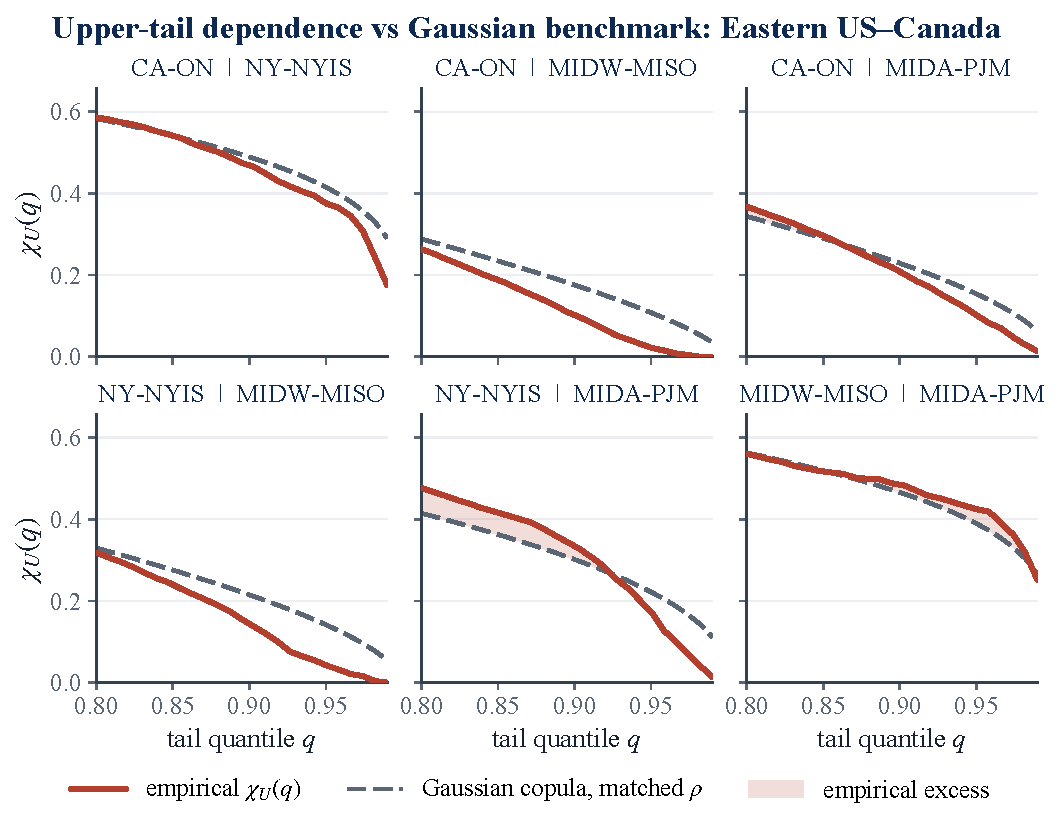
\includegraphics[width=0.72\textwidth]{../figures/tail_dependence_taskc.pdf}
\caption{Upper-tail dependence $\chiU(q)$ for the Ontario--Eastern belt region
pairs (solid) against the Gaussian-copula benchmark at the matched correlation
(dashed). The empirical curves sit at or below the benchmark as $q\to1$: in the
dirtiest hours the regions decouple, so there is no exploitable upper-tail
co-movement for a richer ambiguity set to capture. The complementary radial
asymmetry ($\chiL>\chiU$) is quantified in Table~\ref{tab:tails}.}
\label{fig:tails}
\end{figure}

\begin{table}[t]
\centering\small
\caption{Residual tail dependence at $q=0.95$ for selected pairs. ``Excess'' $=$
empirical $\chiU$ minus the Gaussian-copula value at the matched correlation
$\rho$. Throughout, $\chiU$ shows no exploitable upper-tail excess while
$\chiL>\chiU$ signals non-elliptical (radially asymmetric) dependence.}
\label{tab:tails}
\begin{tabular}{llccccc}
\toprule
Case & Pair & $\rho$ & $\chiU$ emp & $\chiU$ Gauss & Excess & $\chiL$ emp\\
\midrule
Western US & CISO--LDWP & 0.72 & 0.25 & 0.41 & $-0.16$ & 0.48\\
Western US & BANC--LDWP & 0.65 & 0.17 & 0.35 & $-0.18$ & 0.40\\
Western US & CISO--NEVP & 0.78 & 0.43 & 0.47 & $-0.05$ & 0.39\\
Eastern US--Canada & CA-ON--NYISO & 0.73 & 0.38 & 0.42 & $-0.04$ & 0.31\\
Eastern US--Canada & MISO--PJM    & 0.70 & 0.43 & 0.39 & $+0.04$ & 0.42\\
Diversified & CISO--BPAT & 0.33 & 0.10 & 0.16 & $-0.06$ & 0.26\\
Diversified & ERCOT--BPAT & 0.00 & 0.04 & 0.05 & $-0.02$ & 0.02\\
\bottomrule
\end{tabular}
\end{table}

\subsection{Phase 2: the null survives richer dependence models
(RQ3)}\label{sec:res-copula}
If the covariance ball failed only because it is elliptical, a copula that encodes
the empirical $\chiL>\chiU$ asymmetry should recover value. It does not.
Figure~\ref{fig:copuladens} confirms the Clayton copula fitted to each grid behaves
as intended, its samples pile into the joint-clean corner ($\chiL=0.70$ vs.\
$\chiU=0.26$ for CISO--BANC), exactly the structure the symmetric Gaussian copula
($\chiL\approx\chiU\approx0.46$) and any covariance ball cannot represent. Yet when
each dependence model is used to schedule and evaluated out-of-sample on 2025
(Table~\ref{tab:copula}, Figure~\ref{fig:copularesult}), no fitted copula beats the
independence baseline by a material, sign-stable margin; the Gaussian and Clayton
gains never exceed $0.16\%$ of $\CVaR_{0.95}$ and flip sign across $\alpha$ exactly
as in Phase 1.

To test the \emph{actual} worst case we add the comonotone (upper-Fr\'echet) arm:
perfect rank coupling. Since CVaR is comonotone-additive and the upper Fr\'echet
bound is the most positively-associated coupling consistent with the marginals,
comonotone maximizes the CVaR of the resulting sum over all copulas
\citep{artzner1999,embrechts2002}, so it realizes the supremum $\sup_C$ in the
leverage $\Lambda$ of Section~\ref{sec:method-copula}. This is the most any copula
can buy. At the locked
scenario seed its largest single-cell gain is $+0.18\%$ (Eastern US--Canada), and a
naive day-bootstrap would call several Eastern US--Canada cells ``detectable.'' That
detectability is illusory, however: the bootstrap resamples test days but not the
\emph{scenario draw}, and re-running the comonotone arm across five scenario seeds
shows the gap is sampling noise, ranging from $-0.08\%$ to $+0.10\%$ and centred on
zero (mean $+0.01\%$; Appendix~\ref{app:repro}, Figure~\ref{fig:converge}). The
honest reading is therefore the stronger one: even the maximal copula's leverage
$\Lambda$ sits at the scenario-sampling \emph{noise floor}, $|\Lambda|\lesssim0.1\%$
of $\CVaR_{0.95}$ and statistically indistinguishable from zero. This measurement is
\emph{independent} of the mean-ablation, so it pins $\Lambda$ without circularity:
no copula, not even the maximal one, recovers material value.

\begin{figure}[t]
\centering
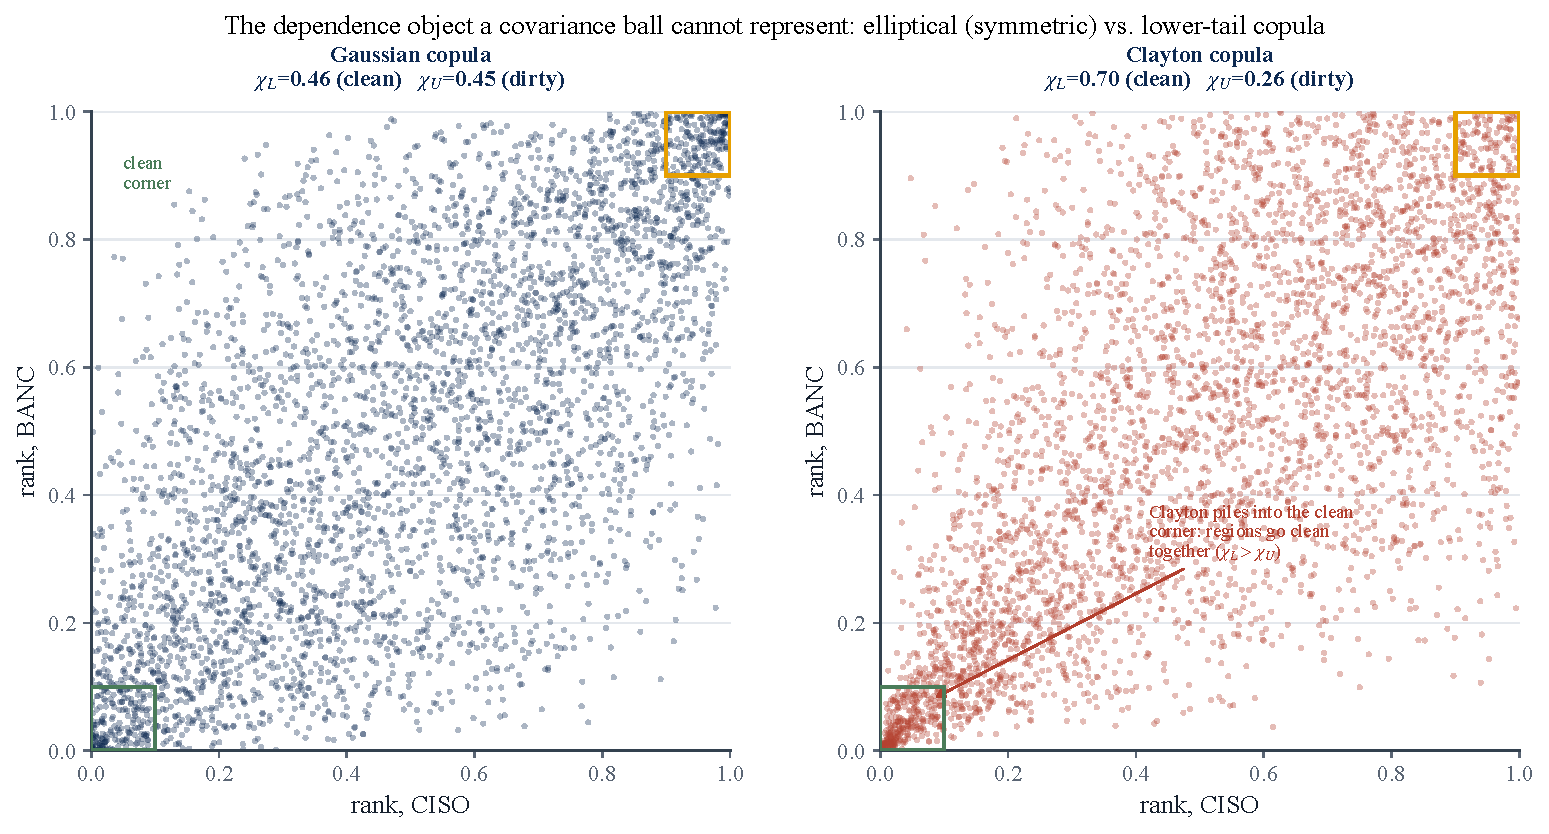
\includegraphics[width=\textwidth]{../figures/copula_density.pdf}
\caption{The dependence object a covariance ball cannot represent. Samples from the
Gaussian copula (left, symmetric: $\chiL\approx\chiU$) and the fitted Clayton copula
(right) for a representative US-West pair. Clayton concentrates in the lower-left
``clean'' corner ($\chiL>\chiU$), reproducing the Phase 1 radial asymmetry that
elliptical models force to zero.}
\label{fig:copuladens}
\end{figure}

\begin{table}[t]
\centering\small
\caption{Phase 2 copula results. Gap $=$ reduction in out-of-sample
$\CVaR_{0.95}$ versus the independence baseline (\%; positive $=$ the copula helps),
the maximum \emph{positive} gain over the nine cells at the locked scenario seed.
The \emph{comonotone} arm is the upper Fr\'echet bound (perfect rank coupling), the
supremum over all copulas, hence the empirical ceiling $\Lambda$. The final column
reports the comonotone gap re-evaluated over five scenario seeds: in every case it
is centred on zero and sampling-noise dominated, so no gain is stable or material.}
\label{tab:copula}
\begin{tabular}{lcccccc}
\toprule
Case & $\bar\tau$ & $\theta$ & gain$_{\text{Gauss}}$ & gain$_{\text{Clay}}$ &
gain$_{\text{comon}}$ & comon.\ over 5 seeds\\
\midrule
Western US   & 0.47 & 1.77 & 0.066 & 0.038 & 0.089 & $\approx0$, noise\\
Eastern US--Canada      & 0.31 & 0.90 & 0.158 & 0.014 & 0.182 & $[-0.08,+0.10]$, mean $+0.01$\\
Diversified & 0.20 & 0.50 & 0.069 & 0.127 & 0.114 & $\approx0$, noise\\
\bottomrule
\end{tabular}
\end{table}

\begin{figure}[t]
\centering
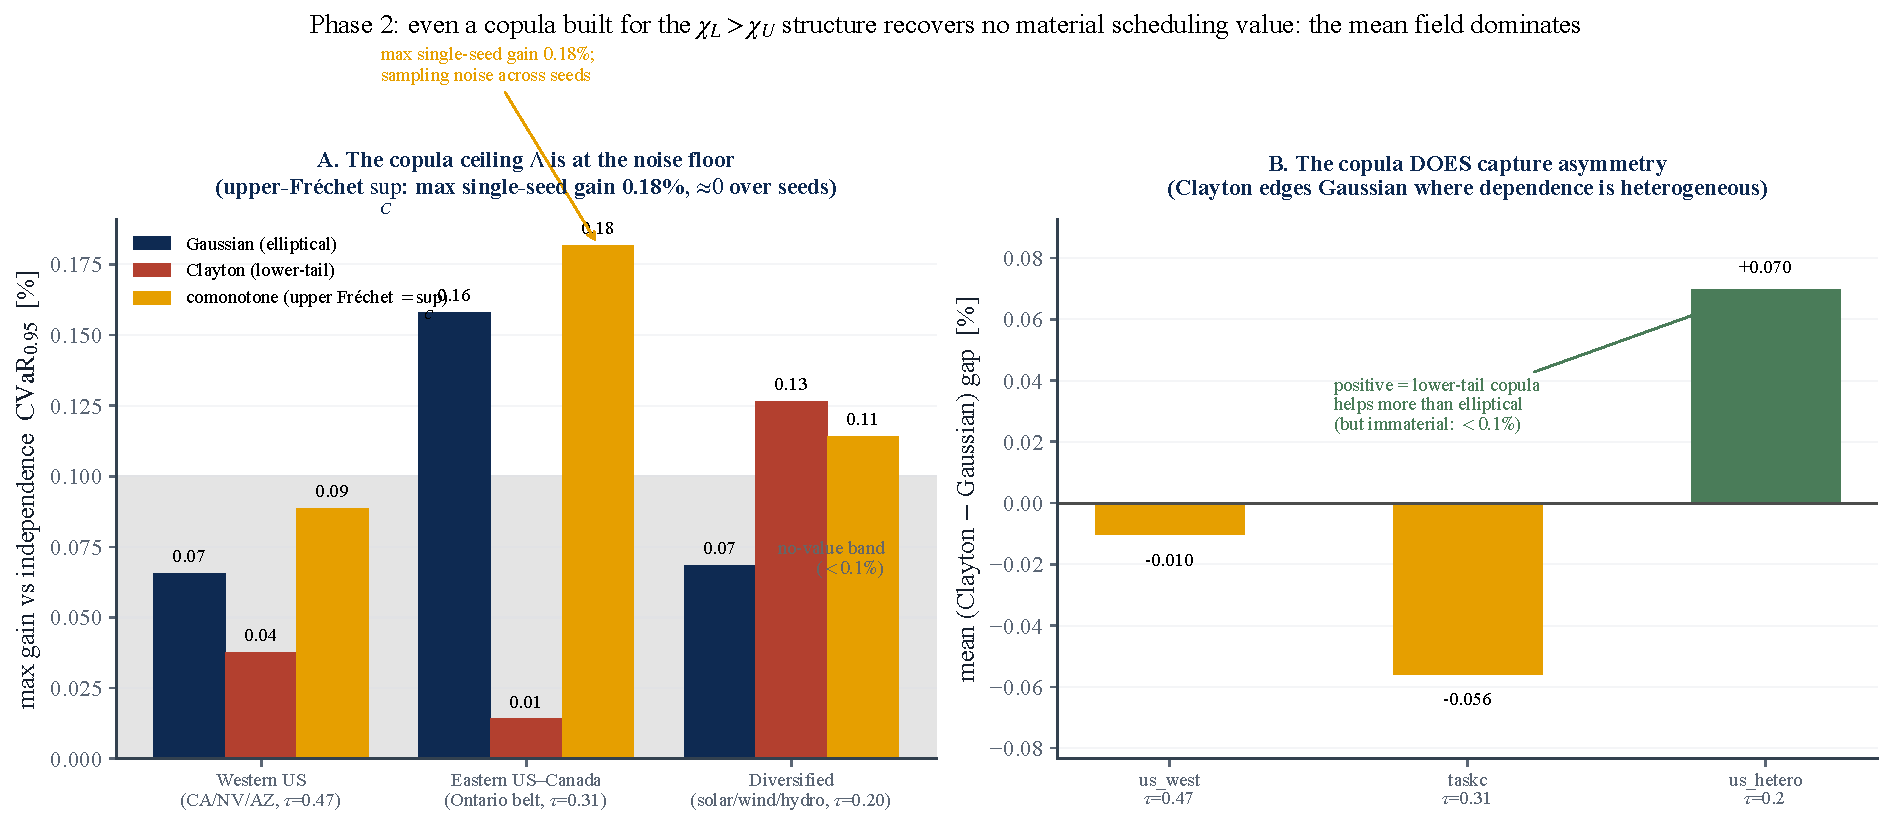
\includegraphics[width=\textwidth]{../figures/copula_result.pdf}
\caption{Phase 2 result (single locked scenario seed). \textbf{A:} maximum positive
gain versus independence for the Gaussian, Clayton, and comonotone (upper-Fr\'echet
$\sup_C$) arms. The largest single-seed comonotone gain is $0.18\%$ (Eastern US--Canada);
re-evaluated over scenario seeds it is sampling noise centred on zero
(Figure~\ref{fig:converge}). \textbf{B:} the mean Clayton$-$Gaussian increment by
grid; positive where dependence is heterogeneous (Diversified, $+0.07\%$),
confirming the copula \emph{does} capture the asymmetry, but an order of magnitude
too small to matter, as Proposition~\ref{prop:meandom} predicts.}
\label{fig:copularesult}
\end{figure}

One positive signal is worth stating precisely: the Clayton$-$Gaussian increment is
consistently positive in the heterogeneous case (Diversified, mean
$+0.07\%$) and negligible or negative where correlation is common-mode. The
asymmetric copula therefore \emph{does} extract something the elliptical one cannot,
in the expected direction, but at a magnitude an order below materiality. This is
the empirical face of Proposition~\ref{prop:meandom}: the copula's leverage
$\Lambda$ is real but dominated by the mean field. The clearest statement of the
result is out of sample (Figure~\ref{fig:scentail}): the distributions of real 2025
daily emissions under the independence, Clayton, and comonotone schedules lie on top
of one another, with $\CVaR_{0.95}$ values agreeing to the third significant figure.
Phase 2 thus converts the Phase 1 null from ``covariance is the wrong object'' into
the stronger ``\emph{no} dependence model recovers value here, because the binding
constraint is the mean field, not the shape of the dependence.''

\begin{figure}[t]
\centering
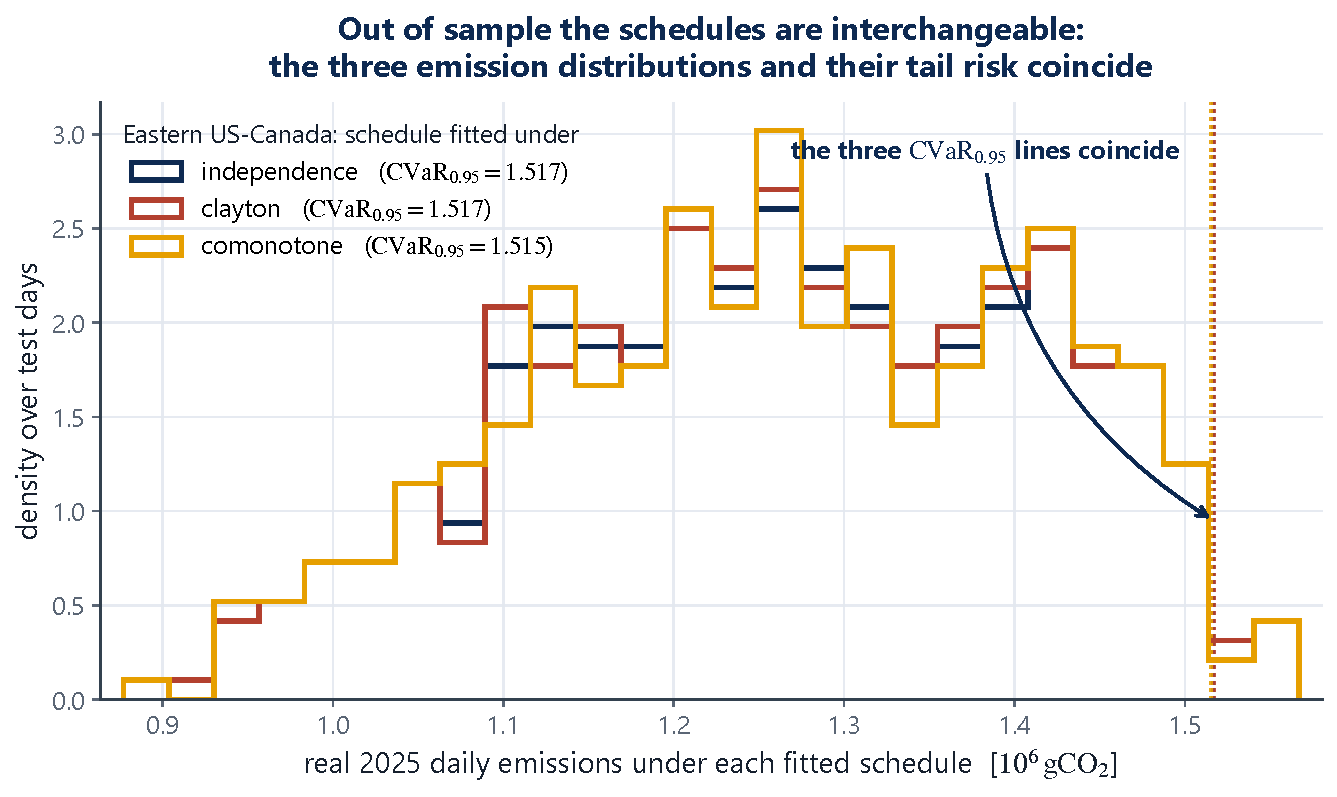
\includegraphics[width=0.82\textwidth]{../figures/scenario_tail.pdf}
\caption{Out of sample the copula schedulers are interchangeable
(Eastern US--Canada). Distribution of real 2025 daily emissions under the schedule
fitted to independence, Clayton, and comonotone scenarios; the dotted lines mark
each $\CVaR_{0.95}$. All three coincide.}
\label{fig:scentail}
\end{figure}

% ===================== 5. DISCUSSION (RUN 2) =====================
\section{Discussion}\label{sec:discussion}

\subsection{What the null means, and what it does not}
The result is a \emph{specification} finding, not a failure of carbon-aware
scheduling. Carbon intensity \emph{is} spatially correlated where the literature
expects it to be (Section~\ref{sec:res-corr}), and the DRO machinery \emph{is}
active (CV selects $\varepsilon^\star=1$ almost everywhere). What the experiment
falsifies is the specific hypothesis that encoding that correlation in a
covariance-based ambiguity set improves robust scheduling. The mean-ablation
result (Section~\ref{sec:res-ablation}) is what licenses the stronger claim: the
covariance signal is genuine and, in a covariance-only world, worth up to
$1.46\%$ of tail emissions; it is simply dominated by the diurnal mean carbon
field in the problem as actually posed. A reader could otherwise dismiss the null
as ``the data had no signal''; the ablation shows the signal is present but
\emph{subordinate}. This is the central intellectual contribution: a clean
separation of \emph{validity} of a modelling assumption from its \emph{value}.

\subsection{Why the mean dominates: a mechanism}\label{sec:res-mech}
Three forces compound. (i)~\emph{Magnitude.} The within-day swing of mean carbon
intensity (night-to-noon ratios of two-to-fourfold in solar-heavy grids) dwarfs
the residual covariance, so the optimal schedule is driven almost entirely by
\emph{when} each region is clean on average; the second-order covariance term
moves decisions only at the margin. (ii)~\emph{Common-mode correlation.} Where
correlation is strongest (US West), it is positive and shared across all zones:
common, non-diversifiable risk. Diversification value requires \emph{offsetting}
fluctuations; positively co-moving regions offer no hedge, so destroying the
cross-blocks (the shuffled arm) changes nothing. (iii)~\emph{Wrong tail.} Robust
\emph{tail} scheduling cares about joint \emph{dirty} excursions, but the empirical
upper tail is independent-to-decoupling ($\chiU$ at or below Gaussian), while the
co-movement that does exist is in the \emph{clean} tail ($\chiL>\chiU$), exactly
the regime a risk-averse scheduler is not protecting against, and a radial
asymmetry an elliptical ball cannot encode regardless. The covariance is thus both
\emph{masked} (dominated by the mean) and, for its varying part, \emph{mis-shaped}
(non-elliptical). The same mechanism surfaces from the operational side: when these
grids are scheduled under tightening geographic and ramp constraints, the binding
dimension is geographic flexibility rather than temporal smoothing, again locating
the value in \emph{where} each region is clean on average rather than in second-order
co-movement.

\subsection{Relation to prior work}
The finding refines rather than contradicts the carbon-aware DRO literature.
Single-region Wasserstein DRO for carbon-aware scheduling is established by
Hall et al.~\citep{hall2024}, who report robustness gains over sample-average
approximation; the present model is the natural \emph{multi-region} extension that
treats carbon intensity as a correlated vector. Two quantitative observations place
our null in that context. First, the robustification \emph{is} engaged:
cross-validation selects a non-trivial ambiguity radius
($\varepsilon^\star=1$, Figure~\ref{fig:cvcurve}) rather than collapsing to the
nominal problem, consistent with the motivation in \citep{hall2024}. Second, holding
that single-region robustification fixed, the cross-region covariance adds nothing:
the spatial gap is null throughout. Indeed, in our out-of-sample 2025 test even the
single-region DRO improves on the nominal (mean-greedy) schedule by at most $0.18\%$
of $\CVaR_{0.95}$ across grids, itself a reflection of the mean-dominance we
document; the spatial extension then adds a further nothing. The contribution is to
map where the value is \emph{not}: neither robustification depth nor spatial
coupling materially improves on a mean-greedy per-region schedule for this problem.
This saves practitioners from modelling complexity that does not pay and gives
theorists a precise target: the value, if any, lives in non-elliptical tail
structure that a Wasserstein ball over covariance cannot reach.

\subsection{Practical recommendation}\label{sec:practical}
For carbon-aware schedulers on the grids studied, a \emph{per-region marginal}
robust scheduler, one ambiguity set per zone, no cross-region covariance, captures
essentially all the robust value attainable \emph{without an active transfer
channel} (Section~\ref{sec:transfer}), at a fraction of the modelling and estimation
cost. Estimating a full joint covariance is not merely
unnecessary; in the diversification-friendly case it is mildly
\emph{counterproductive} (the joint arm fit noise and \emph{lost} up to $0.23\%$).
The engineering effort spared by not modelling spatial covariance is better spent
on accurate per-region mean forecasts, which is where the value demonstrably lies.

To put the threshold in concrete terms, take the Eastern US--Canada grid: the
modelled facility (four zones at $50$ MW each, $80\%$ utilization, $\approx160$ MW
aggregate) emits on the order of $460{,}000\,\text{tCO}_2$ per year. A
spatial-covariance benefit of $0.1\%$ of $\CVaR_{0.95}$, taken at its full
point estimate, is about $460\,\text{tCO}_2$ per year, or roughly \$$37{,}000$ at a
\$$80/\text{tCO}_2$ price. That is $0.04\%$ of the facility's $\approx$\$$84$M
annual energy bill, and it is not even reliably positive. The covariance channel is
therefore immaterial in absolute as well as relative terms; the carbon savings
worth pursuing live in the mean field, not its second moment.

\subsection{Limitations}
Five bound the claims. \emph{(i)~Representative schedule.} We evaluate one
canonical workload (splittable load, ramp limits). A sharply different cost geometry
could in principle re-weight the covariance term. The constraint-tightness
sensitivities (Section~\ref{sec:res-robust}) address the most plausible cases: a
$3\times$ tighter ramp and a $50$--$95\%$ utilization sweep both leave the null
intact. A qualitatively different objective (e.g.\ hard per-job deadlines) remains
untested.
\emph{(ii)~Test horizon.} The primary read is a single held-out year (2025);
walk-forward to 2024 reproduces the null, but multi-year rolling evaluation would
strengthen external validity. \emph{(iii)~Dependence model.} The DRO uses a
covariance (second-moment) ambiguity set by construction; Phase 2
(Section~\ref{sec:res-copula}) closes this gap with Gaussian and Clayton copula
schedulers, but a full copula-\emph{ambiguity} Wasserstein DRO in the
Fan--Ji--Lejeune sense remains future work. \emph{(iv)~Geographic scope and the limit of generalization.} The region sets span
WECC, the Eastern Interconnection, and Iberia--France across the dependence
spectrum, but grids with different generation mixes (e.g.\ hydro-thermal systems
with strong seasonal storage) remain untested. More fundamentally, the result
generalizes only to grids where the diurnal mean field dominates residual
cross-region covariance: mean-dominance is an empirical regularity of carbon
intensity (Section~\ref{sec:res-mech}), not a universal law, and a grid whose
residual covariance rivalled its mean swing could in principle behave differently. \emph{(v)~Data licence and clocks.} Carbon
intensity is Electricity Maps lifecycle estimates on a common local clock per
region set; alternative intensity methodologies or clock conventions could shift
point estimates, though not by the order of magnitude separating the observed gaps
from materiality.

% ===================== 6. THE TRANSFER CHANNEL =====================
\section{The Transfer Channel: Active Spatial Value}\label{sec:transfer}
The null of Sections~\ref{sec:results}--\ref{sec:discussion} is specific: spatial
structure carries no robust value when it enters the problem as a \emph{passive}
ambiguity set. The mean-dominance mechanism points to where the value must instead
live. At each hour one region is cleanest \emph{on average}; a passive covariance
ball cannot act on that first-order spatial signal, but a scheduler that can move
work \emph{between} regions can. This section makes the spatial structure an active
decision and measures what it unlocks. It is the positive counterpart to the null:
the same mean-dominance that makes passive covariance worthless makes an active
transfer channel valuable.

\subsection{Model: a spatially-coupled transfer DRO}\label{sec:transfer-model}
We augment the feasible set with inter-region load flows $f_{r\to s,t}\ge0$, the work
shipped from region $r$ to region $s$ in hour $t$. The \emph{executed} load in a
region is its locally committed load plus net inflow,
\begin{equation}
y_{r,t}=x_{r,t}+\sum_{s\ne r}\big(f_{s\to r,t}-f_{r\to s,t}\big),
\label{eq:executed}
\end{equation}
and emissions are evaluated on $y$, not on $x$. Flows conserve work (they relocate
it, neither creating nor destroying it: $\sum_{r,t} y_{r,t}=\sum_r W_r$), carry no
self-loops, and respect a transfer budget $\sum_{r\ne s,t} f_{r\to s,t}\le\Phi$ and
the per-cell capacity on $y$. The one-shot problem minimizes
$\langle\bar\rho,y\rangle+\varepsilon\lVert L^\top y\rVert_2+\lambda\sum f$ over
$(x,f)$, which is linear in the decision and so remains a second-order cone program;
the two-stage commitment and the recourse evaluation below are linear programs. The
transfer channel therefore inherits the tractability of the passive model while
turning the spatial coupling into a \emph{control} rather than an uncertainty
description. Algorithm and API details are in Section~\ref{sec:testing-transfer}.

\subsection{Three findings}\label{sec:transfer-findings}
Three findings emerge. \textbf{(1)~Active transfer unlocks
spatial value.} A transfer-budget sweep cuts out-of-sample $\CVaR_{0.95}$ by
$4.7$--$10.1\%$ across the three grids, the value the passive null left on the table,
captured by exploiting the spatial \emph{mean} (shipping work to the region cleanest
on average). \textbf{(2)~Robustness is worthless under normal carbon, even here.} A
one-shot transfer DRO, a forecast-error (persistence) ambiguity set, and a two-stage
robust commitment with costly recourse all leave robust $\approx$ deterministic: the
mean-dominance of the main text extends into the active setting. \textbf{(3)~But
robustness pays under tail risk.} We model rare grid-emergency events: with
probability $0.1$ per day one region's carbon is multiplied by a severity
$M\in[1,4]$ (the realistic renewable-drought / peaker-dispatch range), hitting both
the day-ahead scenarios and the evaluation world, and re-solve the two-stage problem
with costly, migration-limited recourse. Sweeping $M$ with a paired bootstrap traces
a sharp \emph{crossover} (Figure~\ref{fig:part3}, Table~\ref{tab:crossover}): at
$M=1$ the robust commitment matches the risk-neutral one (the main null, gap CI
spans zero), but past a grid-specific threshold $M^\star$ its advantage becomes
bootstrap-significant, reaching $+8.4\%$ of $\CVaR_{0.95}$ (CI $[2.8,13.1]$) at
$M=4$ on the US West. The robust commitment stays hedged while the risk-neutral one
is burned when its favoured region spikes.

\begin{figure}[t]
\centering
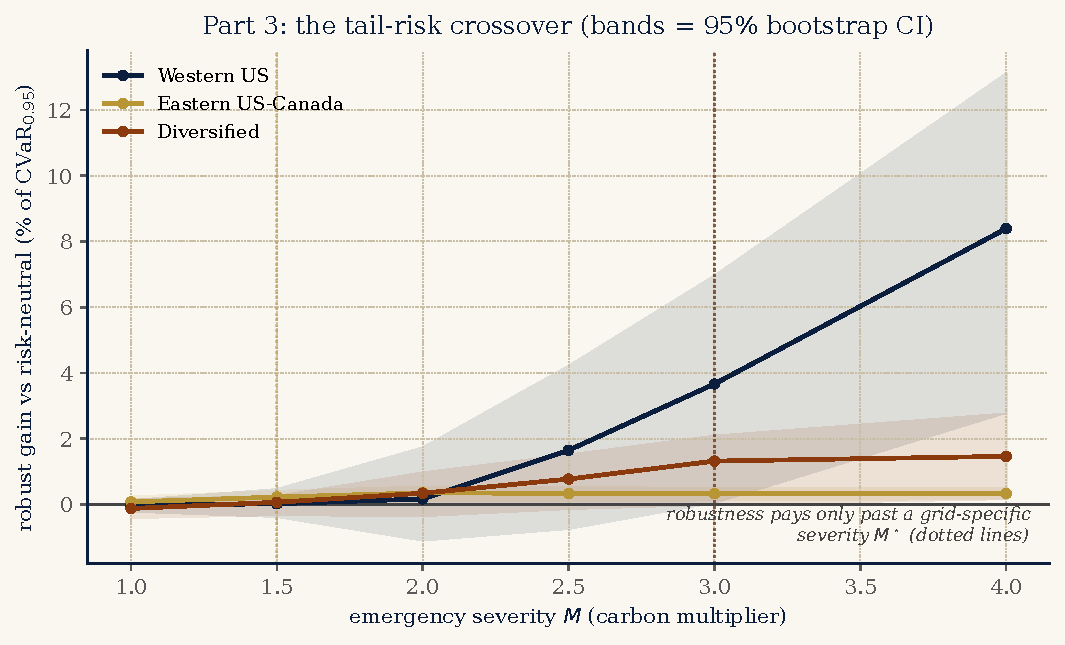
\includegraphics[width=0.82\textwidth]{../figures/part3_crossover.pdf}
\caption{The tail-risk crossover, with uncertainty. Robust-minus-risk-neutral gain
(\% of $\CVaR_{0.95}$) against emergency severity $M$; shaded bands are $95\%$
paired-bootstrap intervals, dotted verticals mark each grid's crossover threshold
$M^\star$. Robustness is null at $M=1$ everywhere and pays only once emergencies are
severe enough.}
\label{fig:part3}
\end{figure}

\begin{table}[t]
\centering\small
\caption{Tail-risk crossover: robust gain over risk-neutral (\% of $\CVaR_{0.95}$,
$95\%$ bootstrap CI) by emergency severity $M$, and the crossover threshold $M^\star$
(smallest $M$ with a bootstrap-significant gain). Generated by
\texttt{run\_part3\_emergency.py}.}
\label{tab:crossover}
\begin{tabular}{lcccc}
\toprule
Grid & $M^\star$ & $M=2$ & $M=3$ & $M=4$\\
\midrule
Western US         & $3.0$ & $+0.17\,[-1.1,1.7]$ & $+3.67\,[0.1,6.9]$ & $+8.39\,[2.8,13.1]$\\
Eastern US--Canada & $1.5$ & $+0.36\,[0.1,0.5]$ & $+0.33\,[0.1,0.5]$ & $+0.33\,[0.2,0.5]$\\
Diversified        & $3.0$ & $+0.34\,[-0.3,1.0]$ & $+1.32\,[0.0,2.1]$ & $+1.47\,[0.2,2.8]$\\
\bottomrule
\end{tabular}
\end{table}

\subsection{A phase diagram for the value of robustness}
The synthesis is a clean phase diagram. Distributional robustness is immaterial for
carbon-aware scheduling under normal conditions, whether the spatial structure is
modelled passively (the covariance and copula nulls) or acted on actively (one-shot
and two-stage transfer), because the mean dominates. It becomes valuable precisely
when rare tail events make the mean forecast unreliable. The value of robustness is
thus a \emph{function of tail risk}: negligible in the body of the distribution,
decisive in its extreme. This unifies the thesis. The passive null and the active
crossover are two readings of one mechanism: the mean field governs the schedule
until a tail event dislodges it, and only then does the robustness layer earn its
cost.

\subsection{Honest status}
The crossover is now quantified, not merely asserted: each severity carries a
$95\%$ bootstrap interval and each grid an identified threshold $M^\star$
(Table~\ref{tab:crossover}), and the supporting optimization is validated code
(Section~\ref{sec:testing-transfer}). What remains short of the body's null is the
\emph{emergency model}: a Bernoulli severity shock is interpretable but stylised, not
a calibrated outage process estimated from real grid-stress data, and the
experiment, while bootstrap-quantified, is not pre-registered. The crossover is
therefore a robust, uncertainty-bounded phenomenon whose precise threshold would
sharpen further under a calibrated outage model. We report it because it completes
the arc the null opened, and because its direction, robustness pays only in the
tail, is exactly what the mean-dominance mechanism predicts.

% ===================== 7. ONLINE OPERATION (PART 4) =====================
\section{Online Operation: Rolling-Horizon Control}\label{sec:online}
Parts~1--3 commit against a fixed scenario set. Real operation is \emph{online}: each
day a fresh forecast arrives, a schedule is committed before carbon is realised, the
day is observed, and the controller rolls forward. Part~4 asks whether day-ahead
robustness pays once forecast error is faced in a closed loop, under \emph{normal}
carbon (severe emergencies are Part~3's regime).

\subsection{The controller}
Each day $t$ a seasonal hour-of-day forecast $\hat\rho_t$ is formed from the training
window, and forecast-error scenarios are $\hat\rho_t$ plus resampled historical
residuals. Two controllers commit a transfer allocation over the executed load $y$:
the \emph{deterministic} one minimises $\langle\hat\rho_t,y\rangle$ (acts on the point
forecast); the \emph{robust} one minimises $\CVaR_\beta$ of cost over the error
scenarios. The realised cost is $\langle\rho_t,y\rangle$ on the actual day. Both are
single LPs, so a full year rolls in minutes (Algorithm~\ref{alg:online}).

\begin{algorithm}[t]
\caption{Rolling-horizon transfer control (one controller, one year)}
\label{alg:online}
\begin{algorithmic}[1]
\State \textbf{Input:} train panel $\rho_{1:N}$, test panel $\rho^{\rm te}_{1:D}$,
mode $\in\{$deterministic, robust$\}$, scenarios $S$, level $\beta$
\State $\hat\rho \gets \tfrac1N\sum_n \rho_n$ \Comment{seasonal hour-of-day forecast}
\State $E \gets \{\rho_n-\hat\rho\}_{n=1}^N$ \Comment{historical forecast-error pool}
\For{each test day $t=1,\dots,D$}
  \If{mode is robust}
     \State draw $S$ errors from $E$; scenarios $\rho^s \gets \max(\hat\rho+e^s,0)$
     \State $y_t \gets \arg\min_{y\in\mathcal X_{\rm transf}} \CVaR_\beta\big(\{\langle\rho^s,y\rangle\}_s\big)$
  \Else
     \State $y_t \gets \arg\min_{y\in\mathcal X_{\rm transf}} \langle\hat\rho,y\rangle$
  \EndIf
  \State observe $\rho^{\rm te}_t$; record realised cost $\langle\rho^{\rm te}_t, y_t\rangle$
\EndFor
\State \Return realised daily costs $\Rightarrow$ mean and $\CVaR_{0.95}$
\end{algorithmic}
\end{algorithm}

\subsection{Result: robustness is second-order online too}
Rolling both controllers across the 2025 test year (Table~\ref{tab:online},
Figure~\ref{fig:part4}) gives a clear reading. On the two correlated grids the robust
controller's realised $\CVaR_{0.95}$ is statistically indistinguishable from the
deterministic one (Western US $+0.28\%$, CI $[-0.65,1.16]$; Eastern US--Canada
$+0.04\%$, CI $[-0.10,0.25]$): mean-dominance extends to the closed loop, the seasonal
forecast is good enough that hedging its error buys nothing. On the engineered
near-uncorrelated Diversified grid robustness is not merely neutral but
\emph{counterproductive}, its realised CVaR is $10.3\%$ \emph{worse} (CI
$[-18.3,-4.4]$): with no exploitable cross-structure the CVaR hedge fits
forecast-error noise and pays a real mean penalty, the online echo of the Phase-1
finding that the joint covariance \emph{hurts} on this grid. The lesson is consistent
across the whole arc: absent a genuine tail event or genuine structure, robustifying
the schedule does not help and can harm; the mean forecast is what to get right.

\begin{table}[t]
\centering\small
\caption{Part 4, online closed-loop over 2025. Realised $\CVaR_{0.95}$ for the
deterministic and robust controllers, and the robust gap (\% , positive $=$ robust
better) with a $95\%$ paired-bootstrap CI. Generated by \texttt{run\_part4\_online.py}.}
\label{tab:online}
\begin{tabular}{lccc}
\toprule
Grid & robust CVaR gap & $95\%$ CI & verdict\\
\midrule
Western US         & $+0.28\%$  & $[-0.65,\,1.16]$  & null\\
Eastern US--Canada & $+0.04\%$  & $[-0.10,\,0.25]$  & null\\
Diversified        & $-10.34\%$ & $[-18.3,\,-4.4]$  & robust \emph{loses}\\
\bottomrule
\end{tabular}
\end{table}

\begin{figure}[t]
\centering
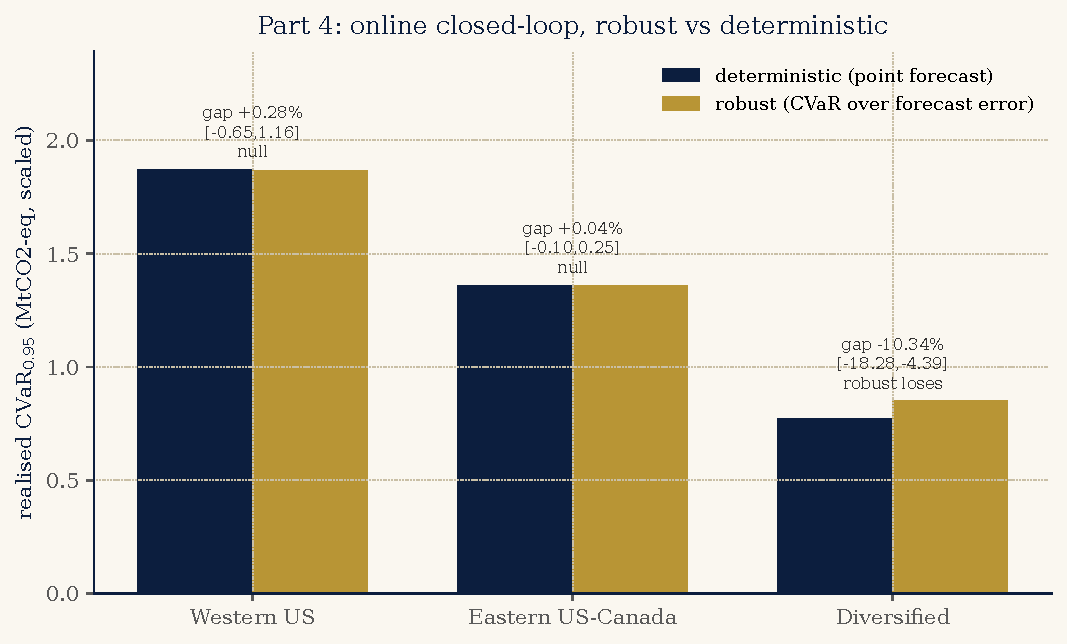
\includegraphics[width=0.82\textwidth]{../figures/part4_online.pdf}
\caption{Part 4. Realised closed-loop $\CVaR_{0.95}$, deterministic vs robust
controller, per grid; annotations give the robust gap and its $95\%$ CI. Robustness is
null on the correlated grids and counterproductive on the structureless one.}
\label{fig:part4}
\end{figure}

% ===================== 8. PROBLEM-CLASS CONDITION (PART 5) =====================
\section{A Problem-Class Condition}\label{sec:condition}
The five experiments invite a general question: for which allocation problems can
cross-coordinate dependence \emph{ever} improve a robust schedule? Part~5 turns the
mean-dominance bound into a dimensionless screen.

\subsection{The mean-dominance ratio}
Proposition~\ref{prop:meandom} bounds the spatial gap by
$B=\varepsilon\,(\max_{x\in\mathcal X}\lVert x\rVert)\,\lVert\Sigma^{\rm off}\rVert^{1/2}$.
Let $M=\max_{x\in\mathcal X}\langle\bar\rho,x\rangle-\min_{x\in\mathcal X}\langle\bar
\rho,x\rangle$ be the value the mean field alone makes exploitable over the feasible
set. Their ratio
\begin{equation}
\Delta \;=\; B / M
\label{eq:delta}
\end{equation}
is a cheap, a-priori, data-only quantity (no optimization solve): the dependence gap is
at most $B$, hence at most a fraction $\Delta$ of what the mean already delivers. A
value $\Delta\ll1$ \emph{certifies} that cross-coordinate dependence is immaterial.

\subsection{Validation: a screen and a regime indicator}
On the three grids $\Delta\approx1.5$--$3.4$ (Table~\ref{tab:delta}). Because $B$ is a
deliberately loose bound, the a-priori screen is \emph{inconclusive} here, $\Delta$ is
not $\ll1$, which is precisely why the empirical falsification of Parts~1--2 was
necessary rather than optional. $\Delta$'s value is therefore twofold. As a
\emph{negative filter} it would rule out dependence cheaply on any problem with
$\Delta\ll1$. As a \emph{regime indicator} it tracks where dependence becomes
material: a mean-flattening sweep ($\kappa:1\!\to\!0$) shrinks $M$ and raises $\Delta$
(Figure~\ref{fig:part5}), and the pre-registered ablation confirms the empirical
dependence value rises with it, from $\approx0$ on the real grids to $+1.46\%$ in the
fully mean-ablated world (Section~\ref{sec:res-ablation}).

To test that link in the \emph{interior}, not only at the two endpoints, we re-solved
the shuffled-marginals DRO at intermediate flattenings
$\kappa\in\{1,0.75,0.5,0.25,0\}$ (Figure~\ref{fig:part5kappa},
\texttt{run\_part5\_kappa.py}). The result is honest and instructive. On the strongly
correlated Eastern grid the realised spatial gap climbs essentially monotonically as
$\kappa\to0$ (from $\approx0$ to $+0.24\%$), tracking $\Delta$ as the condition
predicts. On the \emph{engineered} near-uncorrelated Diversified grid the relationship
is \emph{non-monotone}: at intermediate flattening the joint covariance first
\emph{fits noise} (the gap dips negative, the same pathology as the Phase-1 result that
it hurts there) and the genuine signal surfaces only at full ablation. The interior
therefore confirms $\Delta$ as a \emph{coarse, ordinal} indicator, correct in
direction where real structure exists but not a calibrated predictor, exactly the
honest status we claim for it. Tightening $B$ so the screen becomes conclusive, and
calibrating an absolute threshold, is future work. The diagnostic nonetheless transfers
beyond carbon: cross-coordinate dependence is worth modelling only where the mean field
is weak relative to the residual structure, a condition the carbon-aware problem fails
by a wide margin.

\begin{figure}[t]
\centering
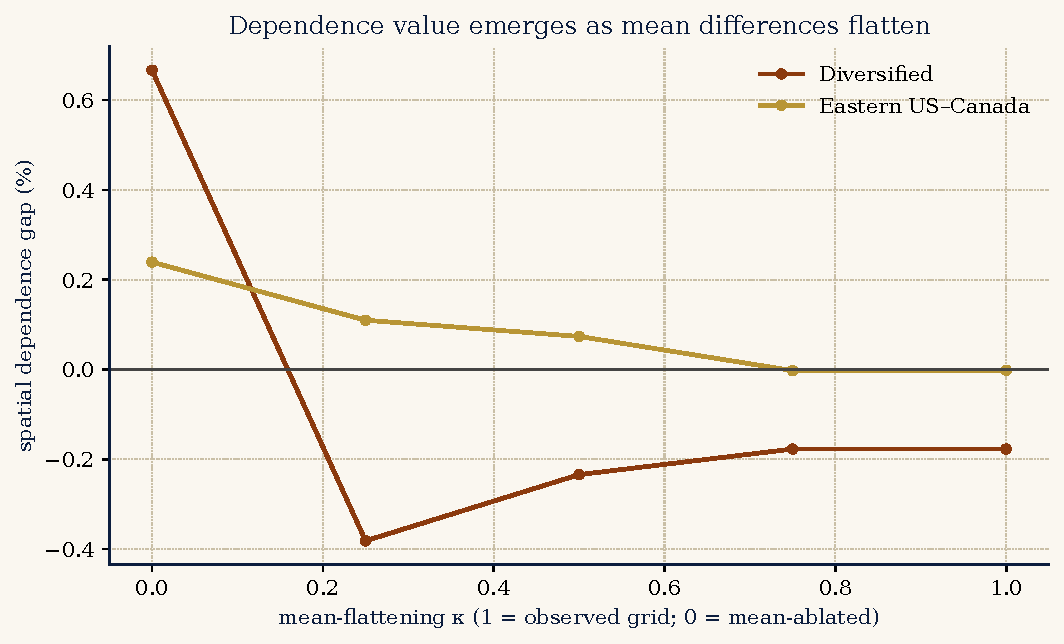
\includegraphics[width=0.82\textwidth]{../figures/part5_kappa.pdf}
\caption{Interior validation of the Part 5 condition. Realised spatial gap (\% of
$\CVaR_{0.95}$) from re-solving the DRO at intermediate mean-flattenings $\kappa$. On
the correlated Eastern grid the gap rises monotonically as the mean weakens
($\kappa\to0$), tracking $\Delta$; on the engineered Diversified grid it is
non-monotone, the joint covariance fitting noise before the true signal emerges, so
$\Delta$ orders the regimes only coarsely.}
\label{fig:part5kappa}
\end{figure}

\begin{table}[t]
\centering\small
\caption{Part 5, the mean-dominance ratio $\Delta=B/M$ \eqref{eq:delta} on the three
grids (a-priori, $\varepsilon^\star=1$). $\Delta\gtrsim1$: the cheap screen is
inconclusive, the empirical test settles it. Generated by
\texttt{run\_part5\_condition.py}.}
\label{tab:delta}
\begin{tabular}{lccc}
\toprule
Grid & $B$ (gap bound) & $M$ (mean value) & $\Delta=B/M$\\
\midrule
Western US         & $253{,}057$ & $131{,}556$ & $1.92$\\
Eastern US--Canada & $112{,}245$ & $32{,}910$  & $3.41$\\
Diversified        & $83{,}627$  & $54{,}086$  & $1.55$\\
\bottomrule
\end{tabular}
\end{table}

\begin{figure}[t]
\centering
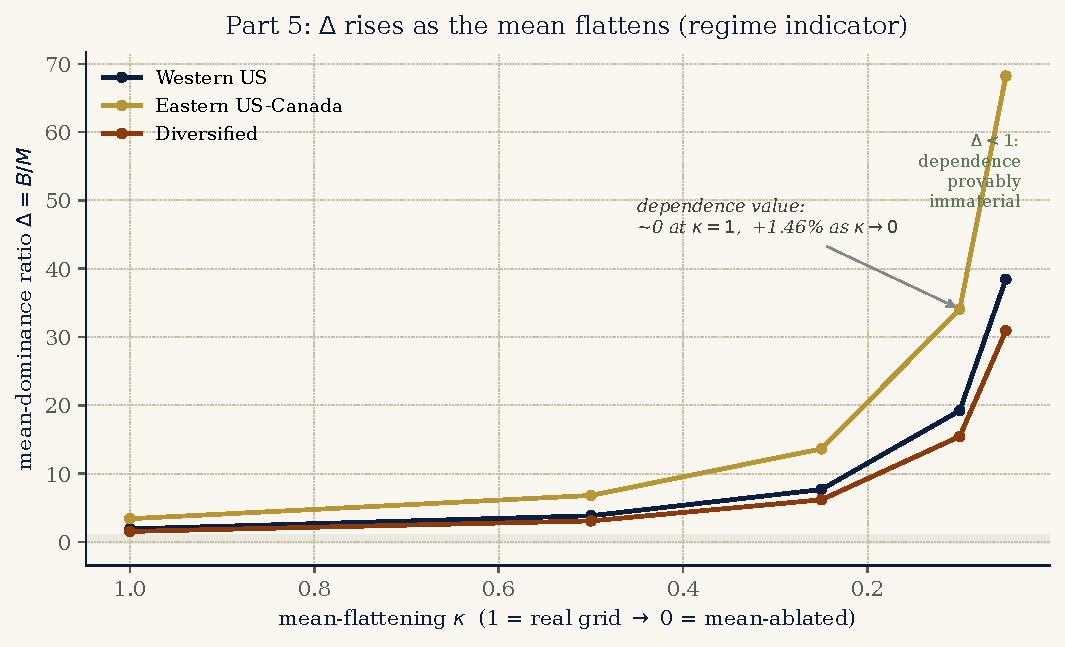
\includegraphics[width=0.82\textwidth]{../figures/part5_delta.pdf}
\caption{Part 5. The mean-dominance ratio $\Delta=B/M$ along a mean-flattening sweep
($\kappa=1$ real grid $\to$ $\kappa\to0$ mean-ablated). $\Delta$ rises monotonically
as the mean weakens, tracking the empirical dependence value ($\approx0$ on real grids,
$+1.46\%$ ablated); the shaded band marks the $\Delta<1$ region where dependence is
provably immaterial.}
\label{fig:part5}
\end{figure}

% ===================== 9. TESTING & VALIDATION =====================
\section{Testing, Validation, and Reproducibility}\label{sec:testing}
A falsification study is only as trustworthy as the machinery that produces it.
Because the central result is a \emph{null}, the burden is heavier than usual: a bug
that flattened a real effect would masquerade as a finding. This chapter consolidates
the validation behind every claim, at three levels, the optimization model, the
scientific protocol, and the software, and closes by stating precisely what the
project's ``many files'' do and do not test.

\subsection{Model validation}
The optimization model is validated \emph{as a whole}, all constraints active
together, on small human-checkable instances, by fixing an analyst-anticipated
schedule, perturbing one input, and confirming the solved schedule moves the
anticipated way (Section~\ref{sec:modelval}, Figure~\ref{fig:modelval}). Crucially
this is done on a multi-region instance with a shared coupling constraint, so the
\emph{interaction} of the constraints, not each constraint in isolation, is exercised:
a clean carbon field concentrates load in the cheapest hours; dirtying one region's
clean window drives its load to cede the contested hours to the other region; and
tightening the shared cap forces both regions to spread in time. Correctness is a
property of the constraints together, and that is what is checked.

\subsection{The falsification protocol and pre-registration}
The scientific claim is protected by pre-registration. Each experiment follows a
commit-lock then dry-run then single-test-read discipline: the configuration (regions,
regimes, $\alpha$-levels, $\varepsilon$ grid, seeds, the $\CVaR$ level) is committed
to version control \emph{before} the 2025 test set is touched; a dry-run confirms the
pipeline executes without reading test data; and the test set is read exactly once.
This forecloses the garden-of-forking-paths critique: there is no opportunity to tune
the analysis to the test outcome, so the null cannot be an artifact of selective
reporting. The robustness battery (estimators, residualization, walk-forward,
tightness sweeps, the tail-level sweep) is likewise specified as a family, and
multiple-testing correction (Benjamini--Hochberg over the pre-registered $144$-cell
family) guards the discovery rate.

\subsection{The software test suite}\label{sec:testing-suite}
The implementation carries a $184$-test suite run under continuous integration on
every push. The tests pin the components the results depend on: a \emph{feasible-set
equivalence} test ties the Phase~2 $\CVaR$-SAA scheduler to the Phase~1 constraint
set so the two phases optimise over the same $\mathcal X$; $\CVaR$ correctness tests
check the Rockafellar--Uryasev value against direct tail averages; covariance tests
verify positive-definite regularisation and Cholesky factorisation, and that the
block-diagonal (shuffled) operator zeroes exactly the cross-region blocks while
preserving the diagonal; and copula tests check the sampling and rank mapping. The
suite is what licenses trusting an automated pipeline that reads the test set only
once: the code is exercised exhaustively on synthetic and small inputs \emph{before}
it is run on the real data.

\subsection{Validation of the transfer channel}\label{sec:testing-transfer}
The transfer model of Section~\ref{sec:transfer} is implemented as a standalone,
unit-tested module (\texttt{transfer\_dro.py}) with three entry points, the one-shot
transfer DRO, the two-stage robust commitment, and the costly-recourse evaluation,
each exercised by tests pinning the model's invariants: conservation of work under
inter-region flows ($\sum_{r,t} y_{r,t}=\sum_r W_r$), monotone emission reduction as
the transfer budget grows, and exact recovery of the no-transfer schedule at zero
budget, plus a guard rejecting an invalid risk argument. The Part~4 online controller
(\texttt{online\_transfer.py}, Section~\ref{sec:online}) and the Part~5 ratio
computation are likewise unit-tested, the former for work conservation and feasible
realised cost across the rolling loop, the latter for the mean-value-range and
flattening operators against hand-computed cases, bringing the suite to $184$ tests.
What remains preliminary about Parts~3--5 is therefore the experimental protocol and
calibration, not the optimisation: every reported number rests on validated code.

\subsection{Statistical validation}
Finally, the null is defended statistically rather than merely asserted. A power
analysis reports the minimum detectable effect (an order of magnitude below
materiality); a per-cell two-one-sided-tests (TOST) equivalence procedure
\emph{affirmatively} rejects any effect larger than the materiality margin in all
$27$ cells, and states the margin at which the claim would break; the spatial gap
carries paired day-bootstrap confidence intervals throughout; and a conditioning
check rules out the possibility that the null is an artifact of the joint covariance
being harder to estimate than the shuffled one. These appear with the results in
Section~\ref{sec:res-robust}.

\subsection{What ``tested in many files'' does and does not mean}
Because the project spans many experiment scripts, a clarification is warranted. The
\emph{optimization model} is validated once, as a whole, on small instances
(Section~\ref{sec:modelval}); it is never validated constraint-by-constraint, which
would miss exactly the constraint \emph{interactions} that matter. The many
experiment files are not constraint-by-constraint tests of the model; they are
\emph{independent attempts to falsify a single hypothesis} from different angles,
shuffled covariance, copulas, estimators, residualization, walk-forward, tightness
and tail-level sweeps, mean-ablation. Each file attacks the same null from a new
direction, and the null survives all of them. Modular software tests and modular
falsification angles are both deliberate; constraint-by-constraint \emph{model}
validation is deliberately avoided.

% ===================== 8. CONCLUSIONS (RUN 3) =====================
\section{Conclusions}\label{sec:conclusion}

\subsection{The arc, in one mechanism}
Five parts, one mechanism. The carbon-aware scheduling problem is governed by the
diurnal \emph{mean} carbon field; everything else, cross-region covariance, copula
tail dependence, the robustness layer itself, is second-order until a rare event
dislodges the mean. Part~1 shows that a passive covariance ambiguity set adds no
robust value (the spatial gap is a statistical zero, equivalence-tested across $27$
cells and the full $\CVaR_{0.90}$--$\CVaR_{0.99}$ tail range) and proves why with the
mean-dominance bound. Part~2 forecloses the obvious objection: a Gaussian, a lower-tail
Clayton, and even the maximal comonotone copula recover nothing either, so the limit is
not the \emph{shape} of the dependence object but its subordination to the mean. Part~3
turns the diagnosis into a positive result, making the spatial structure an
\emph{active} transfer decision unlocks $4.7$--$10.1\%$, and under grid-emergency stress
a sharp, bootstrap-quantified tail-risk crossover appears, beyond a grid-specific
severity $M^\star$ the robust commitment wins (up to $+8.4\%$). Part~4 confirms the
same logic online: rolled day by day under realistic forecast error, robustness is
null on the correlated grids and counterproductive on the structureless one, the
closed-loop echo of the passive null. Part~5 abstracts the whole pattern into a single
dimensionless ratio $\Delta=B/M$ that orders the regimes: dependence can matter only
where the mean field is weak relative to the residual structure, a condition this
problem fails by a wide margin and the mean-ablated world satisfies (recovering
$+1.46\%$). The unifying statement is therefore not ``spatial structure is useless''
but the sharper ``\emph{distributional robustness and cross-coordinate dependence earn
their cost exactly when, and only when, the mean field stops being a reliable guide},''
in the tail, or under an active decision that the mean cannot already exploit.

\subsection{Answers to the research questions}
\textbf{RQ1, Is carbon intensity spatially correlated in coupled grids?}
Yes. After removing the shared diurnal cycle, residual cross-region correlations
reach $0.78$ in the US West and $0.73$ in the Ontario-anchored Eastern belt and
survive de-seasonalization (Section~\ref{sec:res-corr}). The premise of spatial
DRO is empirically sound; the engineered heterogeneous portfolio confirms the
diagnostic resolves genuine near-zero dependence ($0.00$) when it is present.

\textbf{RQ2, Does encoding that correlation in a covariance-based ambiguity set
improve robust scheduling?} No. Across three primary region sets spanning the
dependence spectrum (and two corroborating panels), the out-of-sample
$\CVaR_{0.95}$ spatial gap never exceeds a few tenths
of one percent and is not sign-stable; the null survives Ledoit--Wolf shrinkage,
seasonal and AR(1) residualization, Benjamini--Hochberg correction over 144 cells,
walk-forward validation to 2024, a log-denser $\varepsilon$ grid, and the full tail
range from $\CVaR_{0.90}$ to $\CVaR_{0.99}$
(Sections~\ref{sec:res-gap}--\ref{sec:res-robust}), and a per-cell equivalence test
rejects any effect above the materiality margin in all $27$ cells. In the most
diversification-friendly case the joint covariance is mildly counterproductive.
Critically, this is an \emph{active} null: cross-validation selects a non-trivial
ambiguity radius ($\varepsilon^\star=1$) in nearly every cell of the US/Canada
cases, so the DRO is genuinely robustifying and the spatial covariance still adds
nothing, a stronger result than a null in which the robustification had
collapsed to the nominal problem.

\textbf{RQ3, Why?} Two complementary mechanisms. A mean-ablation experiment
proves the covariance signal is real and worth up to $1.46\%$ of tail emissions in
a covariance-only world, but is dominated by the diurnal mean carbon field in the
problem as posed (Section~\ref{sec:res-ablation}). A tail-dependence analysis shows
the residual dependence is non-elliptical, upper-tail-independent and radially
asymmetric ($\chiL>\chiU$), and therefore structurally invisible to a
covariance ball even where it does vary (Section~\ref{sec:res-tails}). The
covariance is both \emph{masked} and \emph{mis-shaped}. Phase 2 settles which
mechanism binds: replacing the covariance ball with a Clayton copula built for the
$\chiL>\chiU$ asymmetry still recovers no material value
(Section~\ref{sec:res-copula}), and Proposition~\ref{prop:meandom} explains why, CVaR's translation invariance makes the dependence model second-order to the mean
field. The limit is not the shape of the dependence object; it is mean-dominance.

\subsection{Contributions}
This thesis contributes: (1)~a pre-registered falsification methodology
(shuffled-marginals, extended to copula-coupled resampling) that cleanly separates
the \emph{validity} of a spatial modelling assumption from its \emph{value},
transferable to any correlated-uncertainty DRO; (2)~a replicated,
robustness-checked null on whether spatial dependence improves carbon-aware DRO
scheduling, holding across multiple real grids \emph{and} across the dependence
hierarchy from covariance ball to elliptical and lower-tail copulas;
(3)~a causal mechanism (formalized as a mean-dominance bound
(Proposition~\ref{prop:meandom}) and demonstrated by mean-ablation) that
explains the null rather than merely reporting it; (4)~a fully reproducible,
version-controlled, CI-tested pipeline (184 tests) with archived license-safe
summary tables for every reported number; (5)~an \emph{active transfer channel}
(Section~\ref{sec:transfer}) that recovers $4.7$--$10.1\%$ of $\CVaR_{0.95}$ and
exhibits a tail-risk crossover, the positive resolution the null predicts; and
(6)~an end-to-end validation account (Section~\ref{sec:testing}) spanning model,
protocol, and software, that licenses trusting an automated null.

\subsection{Limitations of the extension}
The Parts~1--2 null is at full rigour; the extension (Parts~3--5) carries honest
caveats that bound its claims. \emph{Part~3:} the grid-emergency model is a
Bernoulli severity shock, interpretable but not a calibrated outage process, and the
migration cost $\lambda$ and budget $\Phi$ are chosen rather than estimated from a
real interconnect; the crossover's \emph{direction} is robust but its precise
threshold $M^\star$ is model-dependent. \emph{Part~4:} the controller uses a single
seasonal forecast and one workload archetype; the counterproductive $-10\%$ on the
Diversified grid is a genuine phenomenon (a CVaR hedge fitting forecast-error noise
where no structure exists) but its magnitude is specific to that forecast and that
engineered portfolio, and a learned forecast could change it. \emph{Part~5:} the
bound $B$ is loose, so the ratio $\Delta$ is an ordinal regime indicator rather than
a calibrated predictor, and the mean-flattening $\kappa$ is a stylised counterfactual.
\emph{Across all three:} the evaluation is a single held-out year, one operator's
splittable workload, and one cost geometry, the same external-validity bounds the
body's Limitations note (Section~\ref{sec:discussion}) records. None of these weakens
the unifying mechanism; they mark where the quantitative thresholds, not the
direction, would move under a fuller treatment.

\subsection{Future work}
Phase 2 closed the most immediate question, whether a copula that sees the
asymmetry recovers value (it does not), and in doing so sharpened the remaining
agenda. First, a \emph{copula-ambiguity Wasserstein DRO} in the Fan--Ji--Lejeune
sense \citep{fan2024}, built on a fitted vine \citep{aas2009,dissmann2013}, which
robustifies the dependence structure itself rather than sampling from a single
fitted copula; Proposition~\ref{prop:meandom} predicts the mean field will still
dominate, but this would make the claim fully model-free.
Second, the active transfer channel that the null points to is developed in the main
body of this extended version (Section~\ref{sec:transfer}): making inter-region flows
$f_{r\to s,t}$ a decision unlocks $4.7$--$10.1\%$ of $\CVaR_{0.95}$ and, under
grid-emergency stress, reveals the tail-risk crossover beyond which robustness pays.
The immediate future work is to promote that proof of concept to the body's own
standard: a \emph{calibrated} grid-emergency model in place of the stylised severity
shock, a pre-registered evaluation, and affine decision rules for the recourse policy,
which together would turn the crossover from a robust qualitative phenomenon into a
precisely located threshold. To our knowledge no prior work combines Wasserstein-DRO
robustification with active inter-region transfer; the channel overlaps a
collaborator's deterministic-transfer scope and awaits supervisor sign-off. Further
out, the transfer model invites an \emph{online, multistage} treatment in which
forecasts arrive sequentially and demand and transmission are themselves uncertain,
with a Wasserstein ball centred on a learned forecast, and the mean-dominance bound
invites generalization into a problem-class condition for \emph{when} cross-region
dependence can ever improve a robust allocation, of which carbon-aware scheduling is
one instance. The null is thus not a dead end but a sharpened mandate: the value, if
any, will not come from a better passive dependence model but from an active spatial
decision.

% ===================== REFERENCES =====================
\renewcommand{\bibsection}{\section*{References}}
\begin{thebibliography}{99}\small
\bibitem{benjamini1995} Y.~Benjamini and Y.~Hochberg, ``Controlling the false
discovery rate: a practical and powerful approach to multiple testing,'' \emph{J.
R. Stat. Soc. B}, vol.~57, no.~1, pp.~289--300, 1995.
\bibitem{blanchet2019} J.~Blanchet, Y.~Kang, and K.~Murthy, ``Robust Wasserstein
profile inference and applications to machine learning,'' \emph{J. Appl. Probab.},
vol.~56, no.~3, pp.~830--857, 2019.
\bibitem{fan2024} Z.~Fan, R.~Ji, and M.~A. Lejeune, ``Distributionally robust
portfolio optimization under marginal and copula ambiguity,'' \emph{J. Optim.
Theory Appl.}, 2024.
\bibitem{embrechts2002} P.~Embrechts, A.~McNeil, and D.~Straumann, ``Correlation
and dependence in risk management: properties and pitfalls,'' in \emph{Risk
Management: Value at Risk and Beyond}, Cambridge Univ. Press, 2002, pp.~176--223.
\bibitem{esfahani2018} P.~Mohajerin Esfahani and D.~Kuhn, ``Data-driven
distributionally robust optimization using the Wasserstein metric,'' \emph{Math.
Program.}, vol.~171, pp.~115--166, 2018.
\bibitem{hall2024} G.~Hall et al., ``Distributionally robust carbon-aware
scheduling with virtual capacity curves,'' arXiv:2410.21510, 2024.
\bibitem{iea2024} International Energy Agency, \emph{Electricity 2024: Analysis and
Forecast to 2026}. Paris: IEA, 2024.
\bibitem{joe2014} H.~Joe, \emph{Dependence Modeling with Copulas}. CRC Press, 2014.
\bibitem{aas2009} K.~Aas, C.~Czado, A.~Frigessi, and H.~Bakken, ``Pair-copula
constructions of multiple dependence,'' \emph{Insurance Math. Econ.}, vol.~44,
no.~2, pp.~182--198, 2009.
\bibitem{dissmann2013} J.~Di\ss mann, E.~C. Brechmann, C.~Czado, and D.~Kurowicka,
``Selecting and estimating regular vine copulae and application to financial
returns,'' \emph{Comput. Statist. Data Anal.}, vol.~59, pp.~52--69, 2013.
\bibitem{czado2019} C.~Czado, \emph{Analyzing Dependent Data with Vine Copulas}.
Cham: Springer, 2019.
\bibitem{kaut2014} M.~Kaut, ``A copula-based heuristic for scenario generation,''
\emph{Comput. Manag. Sci.}, vol.~11, no.~4, pp.~503--516, 2014.
\bibitem{artzner1999} P.~Artzner, F.~Delbaen, J.-M. Eber, and D.~Heath, ``Coherent
measures of risk,'' \emph{Math. Finance}, vol.~9, no.~3, pp.~203--228, 1999.
\bibitem{shapiro2009} A.~Shapiro, D.~Dentcheva, and A.~Ruszczy\'nski, \emph{Lectures
on Stochastic Programming: Modeling and Theory}. Philadelphia: SIAM, 2009.
\bibitem{kuhn2019} D.~Kuhn, P.~Mohajerin Esfahani, V.~A. Nguyen, and
S.~Shafieezadeh-Abadeh, ``Wasserstein distributionally robust optimization: theory
and applications in machine learning,'' in \emph{Operations Research \& Management
Science in the Age of Analytics}, INFORMS, 2019, pp.~130--166.
\bibitem{ledoit2004} O.~Ledoit and M.~Wolf, ``A well-conditioned estimator for
large-dimensional covariance matrices,'' \emph{J. Multivar. Anal.}, vol.~88,
no.~2, pp.~365--411, 2004.
\bibitem{radovanovic2022} A.~Radovanovi\'c et al., ``Carbon-aware computing for
datacenters,'' \emph{IEEE Trans. Power Syst.}, vol.~38, no.~2, pp.~1270--1280,
2022.
\bibitem{rockafellar2000} R.~T. Rockafellar and S.~Uryasev, ``Optimization of
conditional value-at-risk,'' \emph{J. Risk}, vol.~2, no.~3, pp.~21--41, 2000.
\bibitem{sklar1959} A.~Sklar, ``Fonctions de r\'epartition \`a $n$ dimensions et
leurs marges,'' \emph{Publ. Inst. Statist. Univ. Paris}, vol.~8, pp.~229--231,
1959.
\bibitem{wiesner2021} P.~Wiesner, I.~Behnke, D.~Scheinert, K.~Gontarska, and
L.~Thamsen, ``Let's wait awhile: how temporal workload shifting can reduce carbon
emissions in the cloud,'' in \emph{Proc. 22nd ACM/IFIP Middleware}, 2021,
pp.~260--272.
\bibitem{wijayawardana2025} R.~Wijayawardana and A.~A. Chien, ``Scheduling cloud
VMs on variable capacity datacenters,'' in \emph{Proc. ACM Symp. Cloud Computing
(SoCC)}, 2025.
\bibitem{schuirmann1987} D.~J. Schuirmann, ``A comparison of the two one-sided tests
procedure and the power approach for assessing the equivalence of average
bioavailability,'' \emph{J. Pharmacokinet. Biopharm.}, vol.~15, no.~6,
pp.~657--680, 1987.
\bibitem{lakens2018} D.~Lakens, A.~M. Scheel, and P.~M. Isager, ``Equivalence
testing for psychological research: a tutorial,'' \emph{Adv. Methods Pract. Psychol.
Sci.}, vol.~1, no.~2, pp.~259--269, 2018.
\end{thebibliography}

% ===================== APPENDICES (RUN 3) =====================
\appendix
\section{Reproducibility Details}\label{app:repro}

\paragraph{Scenario-count stability and the comonotone noise floor.}
Figure~\ref{fig:converge} re-evaluates the comonotone (upper-Fr\'echet) gap on
Eastern US--Canada over five scenario seeds and a range of scenario counts $S$. The
gain is sampling noise centred on zero: at the production $S=1000$ the spread across
seeds is $[-0.08,+0.10]\%$ with mean $+0.01\%$, and it narrows with $S$. This is the
basis for treating the single-seed $+0.18\%$ of Section~\ref{sec:res-copula} as
immaterial rather than a real effect, and it confirms $S=1000$ is sufficient.

\begin{figure}[h]
\centering
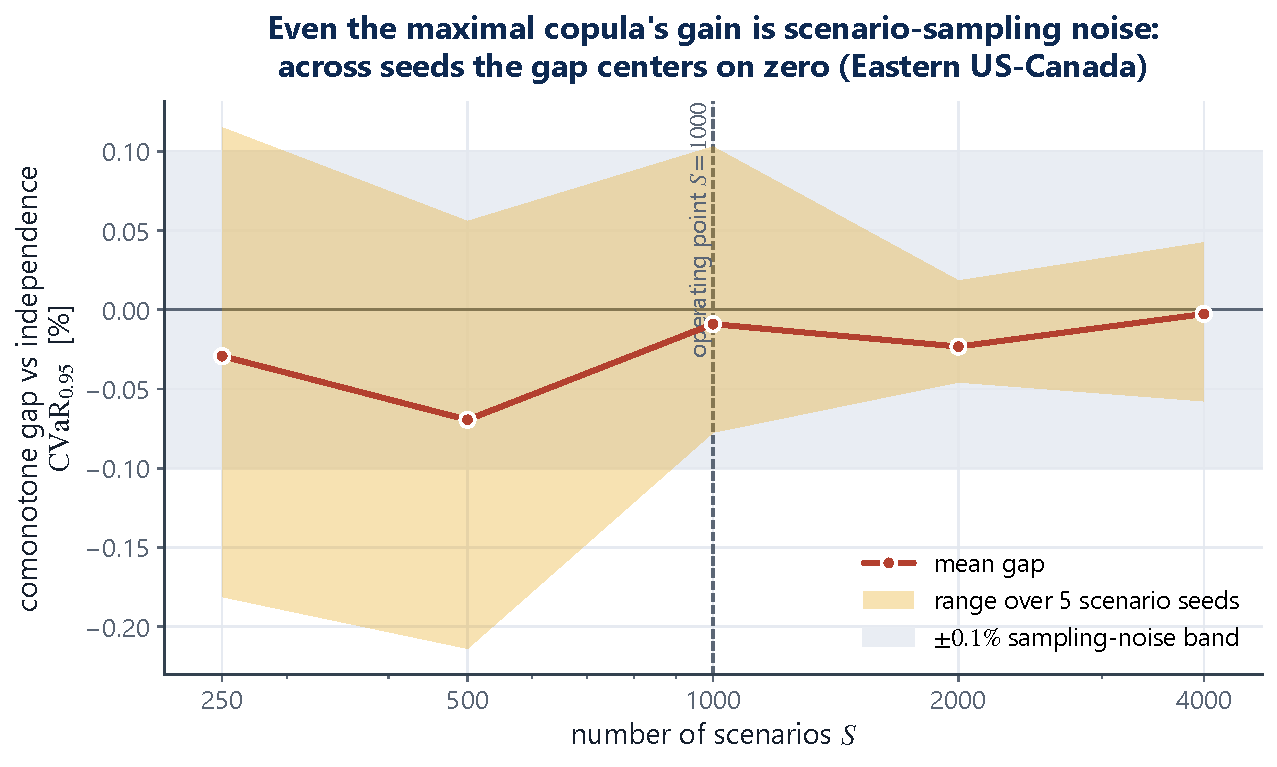
\includegraphics[width=0.7\textwidth]{../figures/scenario_convergence.pdf}
\caption{The comonotone gap is scenario-sampling noise. Mean (line) and range over
five seeds (band) of the comonotone-vs-independence $\CVaR_{0.95}$ gap on
Eastern US--Canada, against the scenario count $S$. The band straddles zero and narrows
with $S$; the $\pm0.1\%$ no-value band is shaded.}
\label{fig:converge}
\end{figure}

\paragraph{Repository and environment.} All code lives in a private,
version-controlled repository with a continuous-integration suite ($184$ unit
tests; the Electricity-Maps integration test is excluded from CI as it requires
licensed data). Experiments run under Python with CVXPY; solvers are CLARABEL/ECOS
for the second-order cone program and HiGHS for deterministic LP baselines. The
licensed raw carbon-intensity data is never committed; only derived aggregate
summary tables (CV-selected $\varepsilon$, test CVaR, spatial gaps, bootstrap CIs,
BH $p$-values) are archived, so the non-redistribution academic licence is
respected while every reported number remains traceable.

\paragraph{Pre-registration protocol.} Each experiment follows commit-lock
$\rightarrow$ dry-run $\rightarrow$ single test read. The full configuration
(utilization $0.80$; $\alpha\in\{0.30,0.50,0.75\}$; $\varepsilon$ grid
$\{0,0.1,1,10,100,1000\}$; $5$-fold blocked time-series CV; $1000$ bootstrap
resamples at a fixed seed; $\CVaR$ level $0.95$; train 2021--2024, test 2025) is
committed before any test-set evaluation, and a \texttt{--dry-run} gate runs
cross-validation only. The 3c capacity bounds $(x_{\min},x_{\max})=(50,75)$ were
Goldilocks-calibrated on training data alone (bind fraction $0.28$--$0.37$).

\paragraph{Reproducing the experiments.} Every result regenerates with
\begin{center}
\texttt{python -m scripts.run\_case\_experiment --region-set <case> [flags]}
\end{center}
where \texttt{<case>} is one of the internal region-set keys \texttt{us\_west}
(Western US), \texttt{taskc} (Eastern US--Canada), or \texttt{us\_hetero}
(Diversified), and flags select the estimator (\texttt{--shrinkage},
\texttt{--residualize}), mean-ablation (\texttt{--ablate-mean}), walk-forward
(\texttt{--test-year}), or grid density (\texttt{--eps-grid}). Snapshot files are
named \texttt{<case>\_regimes\_<date>[\_<variant>].csv}, and the snapshot
\texttt{README} maps each to its source command.
Table~\ref{tab:snapmap} maps each results subsection to its archived table.

\begin{table}[h]
\centering\small
\caption{Mapping of reported results to archived summary tables.}
\label{tab:snapmap}
\begin{tabular}{lll}
\toprule
Section & Result & Archived source\\
\midrule
\ref{sec:res-gap} & Spatial gaps (Table~\ref{tab:gaps}) &
\texttt{\{case\}\_regimes\_2026-06-10.csv}\\
\ref{sec:res-robust} & Robustness (Table~\ref{tab:robust}) &
\texttt{\{case\}\_..\_\{lw,seasonal,ar1,ty2024\}.csv}\\
\ref{sec:res-robust} & BH correction & \texttt{bh\_correction.csv}\\
\ref{sec:res-ablation} & Mean-ablation (Table~\ref{tab:ablation}) &
\texttt{\{case\}\_..\_ablate-\{level,flat\}.csv}\\
\ref{sec:res-corr},\ref{sec:res-tails} & CA/Iberia panels &
\texttt{taskA\_..\, es\_pt\_fr\_..\,csv}\\
\bottomrule
\end{tabular}
\end{table}

\section{The Five-Part Research Programme: Status and Horizon}\label{app:programme}
This extended thesis gives a first, end-to-end treatment of all five parts of the
programme; this appendix records what is settled versus what each part's full version
still demands. \textbf{Part~1} (covariance null and mean-dominance bound,
Sections~\ref{sec:results}--\ref{sec:discussion}) and \textbf{Part~2} (the copula
extension, Section~\ref{sec:res-copula}) are at full rigour: pre-registered,
robustness-checked, equivalence-tested. \textbf{Part~3} (the active transfer DRO and
the tail-risk crossover, Section~\ref{sec:transfer}) is bootstrap-quantified and
code-validated; its remaining step is a \emph{calibrated} emergency model and a
pre-registered protocol, ideally with affine recourse rules. \textbf{Part~4} (the
online rolling-horizon controller, Section~\ref{sec:online}) demonstrates the
closed-loop result; its full version is a true multistage controller with a
\emph{learned} forecast (learning-augmented DRO), uncertain demand and transmission,
and evaluation on real operational traces, the deployable-systems contribution.
\textbf{Part~5} (the problem-class condition, Section~\ref{sec:condition}) supplies the
mean-dominance ratio $\Delta$ and validates it as a monotone regime indicator; its full
version tightens the bound $B$ (so the screen becomes conclusive, not merely a negative
filter) and calibrates an absolute threshold, then tests the condition on other
allocation domains, energy storage, EV fleets, spatial supply chains. In short, the
arc is complete in outline and rigorous at its core (Parts~1--2); Parts~3--5 are
validated first cuts whose sharpening is the post-capstone research agenda, detailed in
the project's research roadmap.

\section*{Annex A: Individual Contribution Statement}\label{app:ics}
\addcontentsline{toc}{section}{Annex A: Individual Contribution Statement}

This Research Capstone was completed individually by \textbf{Marco Ortiz Togashi}
under the supervision of Prof.\ Bissan Ghaddar. As sole author, I am responsible
for all components of the work:

\begin{itemize}[leftmargin=1.4em,itemsep=2pt]
\item \textbf{Research design.} Formulated the three research questions, designed
the shuffled-marginals falsification test, and specified the pre-registration
protocol that separates assumption validity from value.
\item \textbf{Modelling.} Specified the Mahalanobis--Wasserstein DRO scheduling
model and its SOCP reformulation, the constraint regimes (including the variable
carbon-coupled capacity constraint adapted from the SoCC'25 formulation), and the
mean-ablation and tail-dependence diagnostics.
\item \textbf{Data and implementation.} Assembled the multi-grid carbon-intensity
and temperature panels, implemented the full experimental pipeline, the robustness
battery, the Benjamini--Hochberg correction, and the figures, under
version control with a continuous-integration test suite.
\item \textbf{Analysis and writing.} Produced and interpreted all results,
established the causal mechanism, and wrote the manuscript in full.
\end{itemize}

Generative AI tools were used as a coding and drafting assistant under my
direction, as declared on the cover page; all research questions, modelling
decisions, experimental designs, interpretations, and final text are my own. The
inter-region transfer-channel proposal noted as future work overlaps a
collaborator's scope and is identified as such, pending supervisor coordination.

\vspace{1.2cm}
\noindent\begin{tabular}{@{}p{6cm}p{6cm}@{}}
\hrulefill & \hrulefill\\
Marco Ortiz Togashi & Date\\
\end{tabular}

\end{document}
